\PassOptionsToPackage{table,x11names,dvipsnames}{xcolor}

%%%%%%%%%%%%%%%%%%%%%%%%%%%%%%%%%%%%%%%%%%%%%%%%%%%%%%%%%%%%%%%%%%%%%
%% Optimized preamble for achemso SI (cleaned and conflict-free)
%%%%%%%%%%%%%%%%%%%%%%%%%%%%%%%%%%%%%%%%%%%%%%%%%%%%%%%%%%%%%%%%%%%%%
\documentclass[journal=aamick,manuscript=article]{achemso}

% -------------------------------
% --- Encoding and Fonts ---
% -------------------------------
\usepackage[T1]{fontenc}

% -------------------------------
% --- Core math / chemistry ---
% -------------------------------
\usepackage{amsmath,amsfonts}
\usepackage{chemformula} % use \ch{}
\usepackage{amssymb}

% -------------------------------
% --- Graphics and figures ---
% -------------------------------
\usepackage{graphicx}
\graphicspath{{document/}}    % find energy-distribution PDFs
\usepackage{float}            % for [H]
\usepackage[percent]{overpic} % overlay text on figures
\usepackage{tikz}
\usetikzlibrary{arrows.meta, positioning, shapes.geometric, backgrounds, fit}
\usepackage{subcaption}       % provides subfigure environment

% Caption style (subcaption loads caption internally)
\captionsetup{labelfont=bf,font=small}

% -------------------------------
% --- Tables / layout helpers ---
% -------------------------------
\usepackage{booktabs}
\usepackage{array}
\usepackage{makecell}
\usepackage{multirow}
\usepackage{xcolor}
\usepackage{siunitx}
\sisetup{
	output-exponent-marker=\text{e},
	round-mode=figures,
	round-precision=3
}
\usepackage{afterpage}
\setcounter{tocdepth}{2} % 1=Secciones, 2=Subsecciones, 3=Subsubsecciones

% -------------------------------
% --- PDF / landscape pages ---
% -------------------------------
\usepackage{pdflscape}

% -------------------------------
% --- Comments / color tools ---
% -------------------------------
\usepackage{comment}

% -------------------------------
% --- Cross-references ---
% -------------------------------
% NOTE:
% If this file is the SI file (e.g., 00SI.tex), DO NOT point externaldocument to itself.
% Point it to the MAIN manuscript file name (without .tex), and compile the main file first.
\usepackage{xr-hyper} % load before cleveref
\usepackage{cleveref}
% Example:
% \externaldocument[MAIN-]{00Manuscript}
% If you do not need external refs, keep it commented.
% \externaldocument[SI-]{00SI} % <-- do NOT use if this file itself is 00SI.tex
\externaldocument[MAIN-]{main}

% -------------------------------
% --- Line numbering ---
% -------------------------------
\usepackage{lineno}
\setlength\linenumbersep{6pt}
\renewcommand\linenumberfont{\normalfont\tiny}

% -------------------------------
% --- Framed sections (mdframed) ---
% -------------------------------
\usepackage{mdframed}

% Fix mdframed width recalculation warning
\makeatletter
\AtBeginDocument{%
	\setlength{\@tempdima}{\linewidth}%
}
\makeatother

\mdfdefinestyle{breakable}{%
	framemethod=default,
	splittopskip=\baselineskip,
	splitbottomskip=\baselineskip,
	skipabove=\medskipamount,
	skipbelow=\medskipamount
}

% Silence specific mdframed warning
\usepackage{silence}
\WarningFilter{mdframed}{You first box width is too small}

% -------------------------------
% --- Framed sections (tcolorbox) ---
% -------------------------------
\usepackage[skins,breakable]{tcolorbox}

\newtcolorbox{bgblock}[1][]{%
	breakable,
	enhanced,
	width=\linewidth,
	colback=yellow!15,
	colframe=yellow!50!black,
	boxrule=0.2pt,
	sharp corners,
	before upper=\begin{internallinenumbers},
		after upper=\end{internallinenumbers},
	#1
}

% -------------------------------
% --- Spacing ---
% -------------------------------
\usepackage{setspace}
\doublespacing

% -------------------------------
% --- Supplementary Information numbering ---
% -------------------------------
\renewcommand{\thepage}{S-\arabic{page}}
\renewcommand{\theequation}{S-\arabic{equation}}
\renewcommand{\thefigure}{S-\arabic{figure}}
\renewcommand{\thetable}{S-\arabic{table}}
\renewcommand{\thesection}{S-\arabic{section}}

% --- Widen TOC number boxes to accommodate "S-" prefix ---
\usepackage{tocloft}
\setlength{\cftsecnumwidth}{3.2em}      % default ~1.5em; S-## needs more
\setlength{\cftsubsecnumwidth}{4.0em}   % default ~2.3em; S-##.## needs more
\setlength{\cftsubsubsecnumwidth}{5.0em}% default ~3.1em; S-##.##.## needs more
\setlength{\cftsubsecindent}{3.2em}     % align with section numwidth
\setlength{\cftsubsubsecindent}{7.2em}  % subsecindent + subsecnumwidth


%%%%%%%%%%%%%%%%%%%%%%%
%%%  Begin Authors %%%%
%%%%%%%%%%%%%%%%%%%%%%%

\author{Eugenio H. Otal}
\alsoaffiliation{Department of Materials Chemistry, Faculty of Engineering, Shinshu University, 4-17-1 Wakasato, Nagano 380-8553, Japan}
\alsoaffiliation{Research Initiative for Supra-Materials (RISM), Interdisciplinary Cluster for Cutting Edge Research (ICCER), Shinshu University, Nagano 380-8553, Japan}
\alsoaffiliation{Institute for Aqua Regeneration, Shinshu University, 4-17-1 Wakasato, Nagano 380-8553, Japan}
\email{eugenio_otal@shinshu-u.ac.jp}

\author{Manuela L. Kim}
\alsoaffiliation{Department of Materials Chemistry, Faculty of Engineering, Shinshu University, 4-17-1 Wakasato, Nagano 380-8553, Japan}
% \altaffiliation{These authors contributed equally to this work.}

\author{Mutsumi Kimura}
\affiliation{Department of Chemistry and Materials, Faculty of Textile Science and Technology, Shinshu University, Ueda 386-8567, Japan}
\alsoaffiliation{Research Initiative for Supra-Materials (RISM), Interdisciplinary Cluster for Cutting Edge Research (ICCER), Shinshu University, Nagano 380-8553, Japan}
\alsoaffiliation{COI Aqua-Innovation Center, Shinshu University, Ueda 386-8567, Japan}
\alsoaffiliation{Institute for Aqua Regeneration, Shinshu University, 4-17-1 Wakasato, Nagano 380-8553, Japan}

\author{Katsuya Teshima}
\affiliation{Institute for Aqua Regeneration, Shinshu University, 4-17-1 Wakasato, Nagano 380-8553, Japan}
\alsoaffiliation{Department of Materials Chemistry, Faculty of Engineering, Shinshu University, 4-17-1 Wakasato, Nagano 380-8553, Japan}
\alsoaffiliation{Research Initiative for Supra-Materials (RISM), Interdisciplinary Cluster for Cutting Edge Research (ICCER), Shinshu University, Nagano 380-8553, Japan}

\author{Hideki Tanaka}
\affiliation{Institute for Aqua Regeneration, Shinshu University, 4-17-1 Wakasato, Nagano 380-8553, Japan}
\alsoaffiliation{Department of Materials Chemistry, Faculty of Engineering, Shinshu University, 4-17-1 Wakasato, Nagano 380-8553, Japan}
\alsoaffiliation{Research Initiative for Supra-Materials (RISM), Interdisciplinary Cluster for Cutting Edge Research (ICCER), Shinshu University, Nagano 380-8553, Japan}
\email{htanaka@shinshu-u.ac.jp}

\phone{+81 (0)268-21-5499}
\fax{+81 (0)268-21-5499}

\title[Unified Framework for Isotherm Analysis in Water Treatment]
{A Unified Framework for Adsorption Isotherm Analysis in Water Quality Studies: Descriptors, Model Selection, and Reporting Guidelines}

% \abbreviations{IR,NMR,UV}
\keywords{Isotherms,
	Water quality,
	Adsorption }

%%%%%%%%%%%%%%%%%%%%%
%%%  End Authors %%%%
%%%%%%%%%%%%%%%%%%%%%

\SectionNumbersOn

\begin{document}
	
	\linenumbers
	
	\newpage 
	
	\tableofcontents

	
\newpage

\section{Isotherm model equations and limits}
\label{sec:si_models}

This section collects the full equations and limiting behaviors used in
Section~2 of the main manuscript. The availability summary is given in
Table~1 of the main manuscript.

\subsection{Henry isotherm}
\label{sec:si_henry}

The Henry isotherm is the low-coverage limit of many models:
\begin{equation}
	q_e = K_H C_e.
	\label{eq:si_henry_model}
\end{equation}
It has no saturation capacity $Q_{\max}$ and therefore no
model-independent $K_{\mathrm{aff}} = K_H/Q_{\max}$. The Henry constant
$K_H$ is defined by the initial slope.

\paragraph{Low-concentration limit.}
The Henry model is itself the $C_e \to 0$ limit:
\begin{equation}
	\lim_{C_e \to 0} \frac{q_e}{C_e} = K_H.
\end{equation}

\paragraph{High-concentration limit.}
The model is linear and \textbf{does not saturate}, so $q_e \to \infty$ as
$C_e \to \infty$.

\subsection{Langmuir isotherm}
\label{sec:si_langmuir}

The Langmuir isotherm is written as
\begin{equation}
	q_e = \frac{Q_{\max} K_L C_e}{1 + K_L C_e},
	\label{eq:si_langmuir}
\end{equation}
where \(q_e\) is the equilibrium adsorbed amount, \(C_e\) is the
equilibrium concentration in the fluid phase, \(Q_{\max}\) is the maximum
adsorption capacity, and \(K_L\) is the Langmuir equilibrium constant.

\subsubsection{High concentration limit, \(Q_{\max}\): \(C_e \to \infty\)}

From Eq.~\eqref{eq:si_langmuir},
\begin{equation}
	\lim_{C_e \to \infty} q_e
	= \lim_{C_e \to \infty}
	\frac{Q_{\max} K_L C_e}{1 + K_L C_e}
	= Q_{\max}.
\end{equation}
Therefore,
%\noindent\fbox{%
%\parbox{0.97\linewidth}{%
\textbf{Langmuir has finite $Q_{\max}$}:\quad
$\displaystyle \lim_{C_e \to \infty} q_e = Q_{\max}$.%}%
% }

\subsubsection{Low concentration limit: Henry constant}

For small \(C_e\) with \(K_L C_e \ll 1\),
\begin{equation}
	q_e \approx Q_{\max} K_L C_e.
\end{equation}
The Henry law form is
\begin{equation}
	q_e \approx K_H C_e,
	\label{eq:si_henry}
\end{equation}
so the Henry constant is the initial slope:
\begin{equation}
	K_H = \left.\frac{\mathrm{d}q_e}{\mathrm{d}C_e}\right|_{C_e \to 0}
	= Q_{\max} K_L.
\end{equation}
Thus,
\begin{equation}
	\boxed{K_H = Q_{\max} K_L.}
\end{equation}

\subsubsection{Adsorption free energy}

Introduce a standard concentration \(C^0\) and define
\begin{equation}
	K_L^{\ast} = K_L C^0.
\end{equation}
The standard Gibbs free energy of adsorption is
\begin{equation}
	\Delta G_{\mathrm{ads}}^{0}
	= - R T \ln\left( K_L C^0 \right),
\end{equation}
and the corresponding affinity energy is
\begin{equation}
	E_{\mathrm{aff}} = - \Delta G_{\mathrm{ads}}^{0}
	= R T \ln\left( K_L C^0 \right).
\end{equation}
Equivalently,
\begin{equation}
	\boxed{
		\Delta G_{\mathrm{ads}}^{0}
		= - R T \ln\left( K_L C^0 \right),
		\qquad
		E_{\mathrm{aff}} = R T \ln\left( K_L C^0 \right).
	}
\end{equation}

\subsection{Double Langmuir isotherm}
\label{sec:si_double_langmuir}

The dual-site (double) Langmuir isotherm is
\begin{equation}
	q_e
	= \frac{Q_{\max,1} K_1 C_e}{1 + K_1 C_e}
	+ \frac{Q_{\max,2} K_2 C_e}{1 + K_2 C_e},
	\label{eq:si_double_langmuir}
\end{equation}
where \(Q_{\max,i}\) and \(K_i\) are the site capacities and constants.

\subsubsection{High concentration limit: \(C_e \to \infty\)}

For each site,
\begin{equation}
	\lim_{C_e \to \infty} \frac{Q_{\max,i} K_i C_e}{1 + K_i C_e}
	= Q_{\max,i},
\end{equation}
so the total saturation capacity is

\textbf{Double Langmuir has finite }$Q_{\max}$:\quad
$\displaystyle \lim_{C_e \to \infty} q_e = Q_{\max,1} + Q_{\max,2}$.

\subsubsection{Low concentration limit: global Henry constant}

For \(K_i C_e \ll 1\),
\begin{equation}
	q_e \approx Q_{\max,1} K_1 C_e + Q_{\max,2} K_2 C_e,
\end{equation}
which has the Henry form (Eq.~\eqref{eq:si_henry}) with
\begin{equation}
	K_H^{\mathrm{(tot)}}
	= Q_{\max,1} K_1 + Q_{\max,2} K_2.
\end{equation}

\subsubsection{Effective Langmuir constant}

Define \(Q_{\max}^{\mathrm{(tot)}} = Q_{\max,1} + Q_{\max,2}\). Then
\begin{equation}
	K_L^{\mathrm{(tot)}}
	= \frac{K_H^{\mathrm{(tot)}}}{Q_{\max}^{\mathrm{(tot)}}}
	= \frac{Q_{\max,1} K_1 + Q_{\max,2} K_2}
	{Q_{\max,1} + Q_{\max,2}},
\end{equation}
which is a capacity-weighted average of \(K_1\) and \(K_2\).

\subsubsection{Thermodynamic interpretation}

With a standard concentration \(C^0\),
\begin{equation}
	K_i^{\ast} = K_i C^0,
	\qquad
	K_L^{\mathrm{(tot)}\ast} = K_L^{\mathrm{(tot)}} C^0.
\end{equation}
The effective adsorption free energy and affinity are
\begin{equation}
	\Delta G_{\mathrm{ads}}^{0,\mathrm{(tot)}}
	= - R T \ln\left( K_L^{\mathrm{(tot)}} C^0 \right),
	\qquad
	E_{\mathrm{aff}}^{\mathrm{(tot)}}
	= R T \ln\left( K_L^{\mathrm{(tot)}} C^0 \right).
\end{equation}

\subsection{Freundlich isotherm}
\label{sec:si_freundlich}

The Freundlich isotherm is
\begin{equation}
	q_e = K_F C_e^{1/n},
	\label{eq:si_freundlich}
\end{equation}
where \(K_F\) is a capacity-related constant and \(1/n\) is the
heterogeneity exponent.

\subsubsection{High concentration limit: no intrinsic \(Q_{\max}\)}

Taking \(C_e \to \infty\) in Eq.~\eqref{eq:si_freundlich},
\begin{equation}
	\lim_{C_e \to \infty} q_e = \infty.
\end{equation}
Thus, the Freundlich model has no finite saturation capacity:
\begin{equation}
	\boxed{\text{Freundlich has no intrinsic } Q_{\max}.}
\end{equation}

\subsubsection{Low concentration behavior and Henry law}

The derivative of Eq.~\eqref{eq:si_freundlich} is
\begin{equation}
	\frac{\mathrm{d} q_e}{\mathrm{d} C_e}
	= K_F \frac{1}{n} C_e^{1/n - 1}.
\end{equation}
For \(1/n = 1\), the Freundlich model reduces to Henry law with
\(K_H = K_F\). For \(1/n \neq 1\), the initial slope diverges
(\(1/n < 1\)) or vanishes (\(1/n > 1\)) as \(C_e \to 0\).
An apparent, concentration-dependent Henry coefficient can be defined as
\begin{equation}
	K_H(C_e) = \frac{q_e}{C_e}
	= K_F C_e^{1/n - 1}.
\end{equation}

\subsubsection{Affinity constant and apparent free energy}

Using an effective Henry coefficient at a reference concentration
\(C_{\mathrm{ref}}\), one can define
\begin{equation}
	K_{\mathrm{eff}}^{\ast}
	= \left[\frac{1}{n} K_F C_{\mathrm{ref}}^{1/n - 1}\right] C^0,
\end{equation}
leading to an apparent free energy
\begin{equation}
	\Delta G_{\mathrm{ads}}^{0,\mathrm{app}}(C_{\mathrm{ref}})
	= - R T \ln\!\left[
	\frac{1}{n} K_F C_{\mathrm{ref}}^{1/n - 1} C^0 \right].
\end{equation}
This dependence on \(C_{\mathrm{ref}}\) reflects the lack of a unique
free energy for the Freundlich model.

\subsection{Sips (Langmuir--Freundlich) isotherm}
\label{sec:si_sips}

The Sips model introduces a finite saturation capacity while retaining
heterogeneity:
\begin{equation}
	q_e = \frac{Q_{\max} K_S C_e^{m}}{1 + K_S C_e^{m}},
	\label{eq:si_sips}
\end{equation}
where \(0 < m \leq 1\). When \(m = 1\), the model reduces to Langmuir.

\subsubsection{High concentration limit: finite \(Q_{\max}\)}

Taking \(C_e \to \infty\) in Eq.~\eqref{eq:si_sips},
\begin{equation}
	\lim_{C_e \to \infty} q_e = Q_{\max}.
\end{equation}

\subsubsection{Low concentration limit: Freundlich behavior}

For \(K_S C_e^{m} \ll 1\),
\begin{equation}
	q_e \approx Q_{\max} K_S C_e^{m}.
\end{equation}
This has the Freundlich form with
\begin{equation}
	K_F = Q_{\max} K_S,
	\qquad \frac{1}{n} = m.
\end{equation}

\subsubsection{Initial slope and local Henry coefficient}

The low-concentration ratio is
\begin{equation}
	\frac{q_e}{C_e}
	\approx Q_{\max} K_S C_e^{m-1},
\end{equation}
so a local Henry coefficient can be defined as
\begin{equation}
	K_H(C_e) = Q_{\max} K_S C_e^{m - 1},
\end{equation}
which is constant only when \(m = 1\).

\subsubsection{Effective affinity energy}

Define an effective equilibrium constant \(K_{\mathrm{eq}}\) by
\begin{equation}
	\frac{E_0}{RT} = \ln\!\big(K_{\mathrm{eq}}\,C^\circ\big).
	\label{eq:si_E_def}
\end{equation}
For Langmuir, \(K_{\mathrm{eq}} = K_L\), so
\begin{equation}
	\text{Langmuir:}\qquad
	\frac{E_0}{RT} = \ln\!\big(K_L C^\circ\big).
	\label{eq:si_E_langmuir}
\end{equation}
For Sips, the constant \(K_S\) has units \([C]^{-m}\), so an effective
equilibrium constant with units \([C]^{-1}\) is
\begin{equation}
	K_{\mathrm{eq}}^{\mathrm{(Sips)}} = K_S^{1/m}.
\end{equation}
Therefore,
\begin{equation}
	\frac{E_0}{RT}
	= \frac{1}{m}\,\ln\!\big(K_S\,(C^\circ)^{m}\big).
	\label{eq:si_E_sips}
\end{equation}
In the limit \(m = 1\), Eq.~\eqref{eq:si_E_sips} reduces to
Eq.~\eqref{eq:si_E_langmuir}.

\subsection{T\'{o}th isotherm}
\label{sec:si_toth}

The T\'{o}th isotherm is
\begin{equation}
	q_e = \frac{q_{\max}\, b\, C_e}{\left[1 + (b C_e)^t\right]^{1/t}},
	\label{eq:si_toth}
\end{equation}
where $q_{\max}$ is the saturation capacity, $b$ is the affinity
constant, and $0 < t \leq 1$ is the heterogeneity parameter.
When $t = 1$, the model reduces to Langmuir.

\subsubsection{High concentration limit: finite $Q_{\max}$}

As $C_e \to \infty$, $(bC_e)^t \gg 1$, so
\begin{equation}
	\lim_{C_e \to \infty} q_e
	= \lim_{C_e \to \infty}
	\frac{q_{\max}\, b\, C_e}{(b C_e)^{t/t}}
	= q_{\max}.
\end{equation}
% \noindent\fbox{%
%\parbox{0.97\linewidth}{%
\textbf{T\'{o}th has finite }$Q_{\max}$:\quad
$\displaystyle \lim_{C_e \to \infty} q_e = q_{\max}$.%}%
%}

\subsubsection{Low concentration limit: Henry constant}

For $bC_e \ll 1$, $(bC_e)^t \ll 1$ and $[1+(bC_e)^t]^{1/t} \approx 1$, so
\begin{equation}
	q_e \approx q_{\max}\, b\, C_e.
\end{equation}
Therefore,
\begin{equation}
	\boxed{K_H = q_{\max}\, b.}
\end{equation}

\subsubsection{Affinity constant and adsorption free energy}

The affinity constant is $K_{\mathrm{aff}} = b$ (units $[C]^{-1}$). With a standard concentration $C^0$,
\begin{equation}
	K_{\mathrm{aff}}^{\ast} = b\, C^0,
	\qquad
	E_{\mathrm{aff}} = RT\ln(b\, C^0).
\end{equation}
Equivalently,
\begin{equation}
	\boxed{
		\Delta G_{\mathrm{ads}}^{0} = -RT\ln(b\, C^0),
		\qquad
		E_{\mathrm{aff}} = RT\ln(b\, C^0).
	}
\end{equation}

\subsection{Jovanovic isotherm}
\label{sec:si_jovanovic}

The Jovanovic isotherm is
\begin{equation}
	q_e = q_{\max}\,\bigl[1 - \exp(-b\, C_e)\bigr].
	\label{eq:si_jovanovic}
\end{equation}

\subsubsection{High concentration limit: finite $Q_{\max}$}

As $C_e \to \infty$, $\exp(-bC_e) \to 0$, so
\begin{equation}
	\lim_{C_e \to \infty} q_e = q_{\max}.
\end{equation}
\textbf{Jovanovic has finite }$Q_{\max}$:\quad
$\displaystyle \lim_{C_e \to \infty} q_e = q_{\max}$.

\subsubsection{Low concentration limit: Henry constant}

For $bC_e \ll 1$, $\exp(-bC_e) \approx 1 - bC_e$, so
\begin{equation}
	q_e \approx q_{\max}\, b\, C_e.
\end{equation}
Therefore,
\begin{equation}
	\boxed{K_H = q_{\max}\, b.}
\end{equation}

\subsubsection{Affinity constant and adsorption free energy}

The affinity constant is $K_{\mathrm{aff}} = b$. With a standard concentration $C^0$,
\begin{equation}
	\boxed{
		K_{\mathrm{aff}}^{\ast} = b\, C^0,
		\qquad
		E_{\mathrm{aff}} = RT\ln(b\, C^0).
	}
\end{equation}

\subsection{Temkin isotherm}
\label{sec:si_temkin}

The Temkin isotherm is
\begin{equation}
	q_e = \frac{RT}{b_T}\,\ln(a_T\, C_e).
	\label{eq:si_temkin}
\end{equation}

\subsubsection{High concentration limit: no intrinsic $Q_{\max}$}

As $C_e \to \infty$, $\ln(a_T C_e) \to \infty$, so
\begin{equation}
	\lim_{C_e \to \infty} q_e = \infty.
\end{equation}
\begin{equation}
	\boxed{\text{Temkin has no intrinsic } Q_{\max}.}
\end{equation}
The Temkin model is valid only over an intermediate concentration range where the linear-in-$\ln C_e$ approximation holds.

\subsubsection{Low concentration limit: no finite Henry constant}

The derivative is
\begin{equation}
	\frac{\mathrm{d}q_e}{\mathrm{d}C_e} = \frac{RT}{b_T\, C_e},
\end{equation}
which diverges as $C_e \to 0$. Therefore,
\begin{equation}
	\boxed{\text{Temkin has no finite } K_H.}
\end{equation}

\subsubsection{Effective affinity constant and adsorption free energy}

An effective affinity constant is defined from the binding constant $a_T$ (units $[C]^{-1}$):
\begin{equation}
	K_{\mathrm{aff}} = a_T,
	\qquad
	K_{\mathrm{aff}}^{\ast} = a_T\, C^0.
\end{equation}
The adsorption free energy is
\begin{equation}
	\boxed{
		E_{\mathrm{aff}} = RT\ln(a_T\, C^0).
	}
\end{equation}
Note that this is an \emph{effective} energy; the Temkin model describes the mid-coverage regime and does not correspond to a well-defined thermodynamic equilibrium constant.

\subsection{UNILAN isotherm}
\label{sec:si_unilan}

The UNILAN isotherm (uniform-energy Langmuir) is
\begin{equation}
	q_e = \frac{Q_{\max}}{2s}
	\ln\!\left(
	\frac{1 + b_{\max}\, C_e}{1 + b_{\min}\, C_e}
	\right),
	\label{eq:si_unilan}
\end{equation}
where $s = \tfrac{1}{2}\ln(b_{\max}/b_{\min})$ is the half-width of the uniform energy distribution.

\subsubsection{High concentration limit: finite $Q_{\max}$}

As $C_e \to \infty$, $b_{\max}C_e \gg 1$ and $b_{\min}C_e \gg 1$, so
\begin{equation}
	q_e \approx \frac{Q_{\max}}{2s}
	\ln\!\left(\frac{b_{\max}}{b_{\min}}\right)
	= \frac{Q_{\max}}{2s} \cdot 2s = Q_{\max}.
\end{equation}
\textbf{UNILAN has finite }$Q_{\max}$:\quad
$\displaystyle \lim_{C_e \to \infty} q_e = Q_{\max}$.

\subsubsection{Low concentration limit: Henry constant}

For $b_{\max}C_e \ll 1$ and $b_{\min}C_e \ll 1$,
$\ln(1+x) \approx x$, so
\begin{equation}
	q_e \approx \frac{Q_{\max}}{2s}(b_{\max} - b_{\min})\, C_e.
\end{equation}
Therefore,
\begin{equation}
	\boxed{K_H = \frac{Q_{\max}}{2s}(b_{\max} - b_{\min}).}
\end{equation}

\subsubsection{Affinity constant and adsorption free energy}

The natural affinity constant is the geometric mean of the site constants:
\begin{equation}
	K_{\mathrm{aff}} = \sqrt{b_{\max}\, b_{\min}},
	\qquad
	K_{\mathrm{aff}}^{\ast} = \sqrt{b_{\max}\, b_{\min}}\; C^0.
\end{equation}
The adsorption free energy is
\begin{equation}
	\boxed{
		E_{\mathrm{aff}} = RT\ln\!\left(\sqrt{b_{\max}\, b_{\min}}\; C^0\right)
		= \frac{RT}{2}\ln\!\left(b_{\max}\, b_{\min}\, (C^0)^2\right).
	}
\end{equation}

\subsection{Redlich--Peterson isotherm}
\label{sec:si_redlich_peterson}

The Redlich--Peterson isotherm is
\begin{equation}
	q_e = \frac{K_{RP}\, C_e}{1 + a_{RP}\, C_e^{\beta}},
	\label{eq:si_redlich_peterson}
\end{equation}
with $0 < \beta \leq 1$.

\subsubsection{High concentration limit: conditional $Q_{\max}$}

As $C_e \to \infty$,
\begin{equation}
	q_e \approx \frac{K_{RP}}{a_{RP}}\, C_e^{1-\beta}.
\end{equation}
If $\beta = 1$ (Langmuir limit): $Q_{\max} = K_{RP}/a_{RP}$ (finite).
If $\beta < 1$: $q_e \to \infty$ (no finite saturation).
\begin{equation}
	\boxed{Q_{\max} = K_{RP}/a_{RP} \quad (\text{only if } \beta = 1).}
\end{equation}

\subsubsection{Low concentration limit: Henry constant}

For $a_{RP}C_e^{\beta} \ll 1$,
\begin{equation}
	q_e \approx K_{RP}\, C_e.
\end{equation}
Therefore, regardless of $\beta$,
\begin{equation}
	\boxed{K_H = K_{RP}.}
\end{equation}

\subsubsection{Affinity constant and adsorption free energy}

Two effective affinity constants are commonly used:
\begin{itemize}
	\item Henry regime: $K_{\mathrm{aff}} = K_{RP}/Q_{\max} = a_{RP}$ (when $\beta=1$).
	\item High-$C$ regime: $K_{\mathrm{aff}} = (a_{RP})^{1/\beta}$.
\end{itemize}
For the purpose of cross-model comparison, we adopt the Henry-based definition:
\begin{equation}
	\boxed{
		K_{\mathrm{aff}}^{\ast} = \frac{K_{RP}}{Q_{\max}}\, C^0
		= a_{RP}\, C^0 \quad (\beta=1),
		\qquad
		E_{\mathrm{aff}} = RT\ln(a_{RP}\, C^0).
	}
\end{equation}

\subsection{Koble--Corrigan isotherm}
\label{sec:si_koble_corrigan}

The Koble--Corrigan isotherm is
\begin{equation}
	q_e = \frac{A_{KC}\, C_e^{1/n}}{1 + B_{KC}\, C_e^{1/n}}.
	\label{eq:si_koble_corrigan}
\end{equation}
This is algebraically equivalent to the Sips isotherm with the identifications
$Q_{\max} = A_{KC}/B_{KC}$, $K_S = B_{KC}$, and $m = 1/n$.

\subsubsection{High concentration limit: finite $Q_{\max}$}

As $C_e \to \infty$, $B_{KC}C_e^{1/n} \gg 1$, so
\begin{equation}
	\lim_{C_e \to \infty} q_e = \frac{A_{KC}}{B_{KC}}.
\end{equation}
\begin{equation}
	\boxed{Q_{\max} = A_{KC}/B_{KC}.}
\end{equation}

\subsubsection{Low concentration limit: conditional Henry constant}

For $B_{KC}C_e^{1/n} \ll 1$,
\begin{equation}
	q_e \approx A_{KC}\, C_e^{1/n}.
\end{equation}
A finite $K_H$ exists only when $1/n = 1$: $K_H = A_{KC}$.
For $1/n \neq 1$, the initial slope is concentration dependent.

\subsubsection{Affinity constant and adsorption free energy}

By analogy with Sips, the effective affinity constant is
$K_{\mathrm{aff}} = B_{KC}^{\,n}$, so
\begin{equation}
	\boxed{
		K_{\mathrm{aff}}^{\ast} = B_{KC}^{\,n}\, C^0,
		\qquad
		E_{\mathrm{aff}} = nRT\ln(B_{KC}\, C^0).
	}
\end{equation}

\subsection{Radke--Prausnitz isotherm}
\label{sec:si_radke_prausnitz}

The Radke--Prausnitz isotherm is
\begin{equation}
	q_e = \frac{a_{RP}\, r_{RP}\, C_e}{a_{RP} + r_{RP}\, C_e^{1-p}},
	\label{eq:si_radke_prausnitz}
\end{equation}
with $0 < p \leq 1$.

\subsubsection{High concentration limit: conditional $Q_{\max}$}

As $C_e \to \infty$, for $p < 1$:
\begin{equation}
	q_e \approx \frac{a_{RP}\, r_{RP}}{r_{RP}}\, C_e^{p} = a_{RP}\, C_e^{p} \to \infty.
\end{equation}
For $p = 1$: $q_e \to a_{RP}\, r_{RP}/(a_{RP} + r_{RP}) \cdot C_e$, which also diverges.
\begin{equation}
	\boxed{\text{Radke--Prausnitz has no intrinsic } Q_{\max} \text{ for } p < 1.}
\end{equation}

\subsubsection{Low concentration limit: Henry constant}

For small $C_e$, $r_{RP}C_e^{1-p} \ll a_{RP}$, so
\begin{equation}
	q_e \approx r_{RP}\, C_e.
\end{equation}
Therefore,
\begin{equation}
	\boxed{K_H = r_{RP}.}
\end{equation}

\subsubsection{Effective affinity constant and adsorption free energy}

Since no unique $Q_{\max}$ exists, the affinity constant is defined directly from the Henry constant:
\begin{equation}
	\boxed{
		K_{\mathrm{aff}}^{\ast} = r_{RP}\, C^0,
		\qquad
		E_{\mathrm{aff}} = RT\ln(r_{RP}\, C^0).
	}
\end{equation}
This is an \emph{effective} energy valid in the low-concentration regime.

\subsection{Dubinin--Radushkevich (D-R) and Dubinin--Astakhov (D-A)}
\label{sec:si_dr_da}

The D-R/D-A isotherms are
\begin{equation}
	q_e = Q_{\max}\,\exp\!\left[-\left(\frac{\varepsilon}{E_a}\right)^{n_{DA}}\right],
	\qquad
	\varepsilon = RT\ln\!\left(1 + \frac{1}{C_e}\right).
	\label{eq:si_dr_da}
\end{equation}
The D-R model corresponds to $n_{DA} = 2$.

\subsubsection{High concentration limit: finite $Q_{\max}$}

As $C_e \to \infty$, $\varepsilon = RT\ln(1+1/C_e) \to 0$, so
$\exp[-(\varepsilon/E_a)^{n_{DA}}] \to 1$ and
\begin{equation}
	\lim_{C_e \to \infty} q_e = Q_{\max}.
\end{equation}
\textbf{D-R/D-A has finite }$Q_{\max}$:\quad
$\displaystyle \lim_{C_e \to \infty} q_e = Q_{\max}$.

\subsubsection{Low concentration limit: no finite Henry constant}

As $C_e \to 0$, $\varepsilon \to \infty$, so
$\exp[-(\varepsilon/E_a)^{n_{DA}}] \to 0$ faster than any power of $C_e$. The derivative
\begin{equation}
	\frac{\mathrm{d}q_e}{\mathrm{d}C_e}
	= Q_{\max}\, \frac{n_{DA}}{E_a}
	\left(\frac{\varepsilon}{E_a}\right)^{n_{DA}-1}
	\exp\!\left[-\left(\frac{\varepsilon}{E_a}\right)^{n_{DA}}\right]
	\cdot \frac{RT}{C_e(1+C_e)}
\end{equation}
diverges as $C_e \to 0$.
\begin{equation}
	\boxed{\text{D-R/D-A has no finite } K_H.}
\end{equation}

\subsubsection{Effective affinity constant and adsorption free energy}

An effective affinity constant is defined from the half-loading concentration $C_{1/2}$
(the concentration at which $q_e = Q_{\max}/2$).
Setting $q_e = Q_{\max}/2$ gives $\varepsilon_{1/2} = E_a(\ln 2)^{1/n_{DA}}$, and
\begin{equation}
	C_{1/2} = \frac{1}{\exp(\varepsilon_{1/2}/RT) - 1}.
\end{equation}
The effective affinity constant and energy are
\begin{equation}
	\boxed{
		K_{\mathrm{aff}} = 1/C_{1/2},
		\qquad
		K_{\mathrm{aff}}^{\ast} = C^0/C_{1/2},
		\qquad
		E_{\mathrm{aff}} = RT\ln(C^0/C_{1/2}).
	}
\end{equation}

\subsection{Hill isotherm}
\label{sec:si_hill}

The Hill isotherm is
\begin{equation}
	q_e = Q_{\max}\,\frac{C_e^{n_H}}{K_D + C_e^{n_H}},
	\label{eq:si_hill}
\end{equation}
where $n_H$ is the Hill coefficient and $K_D$ is the dissociation constant.
When $n_H = 1$, the model reduces to Langmuir with $K_L = 1/K_D$.

\subsubsection{High concentration limit: finite $Q_{\max}$}

As $C_e \to \infty$, $C_e^{n_H} \gg K_D$, so
\begin{equation}
	\lim_{C_e \to \infty} q_e = Q_{\max}.
\end{equation}
\textbf{Hill has finite }$Q_{\max}$:\quad
$\displaystyle \lim_{C_e \to \infty} q_e = Q_{\max}$.

\subsubsection{Low concentration limit: conditional Henry constant}

For $C_e^{n_H} \ll K_D$,
\begin{equation}
	q_e \approx \frac{Q_{\max}}{K_D}\, C_e^{n_H}.
\end{equation}
A finite $K_H$ exists only when $n_H = 1$:
\begin{equation}
	K_H = Q_{\max}/K_D \quad (n_H = 1).
\end{equation}
For $n_H \neq 1$, the initial slope is concentration dependent:
\begin{equation}
	K_H(C_e) = \frac{Q_{\max}}{K_D}\, C_e^{n_H - 1}.
\end{equation}

\subsubsection{Affinity constant and adsorption free energy}

The effective affinity constant with units $[C]^{-1}$ is
$K_{\mathrm{aff}} = K_D^{-1/n_H}$. Therefore,
\begin{equation}
	K_{\mathrm{aff}}^{\ast} = K_D^{-1/n_H}\, C^0,
\end{equation}
and the adsorption free energy is
\begin{equation}
	\boxed{
		E_{\mathrm{aff}} = RT\!\left(-\frac{1}{n_H}\ln K_D + \ln C^0\right).
	}
\end{equation}
In the limit $n_H = 1$, this reduces to the Langmuir expression
$E_{\mathrm{aff}} = RT\ln(K_L\, C^0)$ with $K_L = 1/K_D$.
	

	
% =====================================================================
%  SECTION S-3: ERROR METRICS AND INFORMATION CRITERIA
% =====================================================================
\section{Error metrics and information criteria}
\label{sec:si_error_metrics}

\subsection{Residual error metrics}
\label{sec:si_residuals}

Let the residual at point $i$ be
\begin{equation}
	r_i = q_i^{\exp} - q_i^{\mathrm{pred}}(\boldsymbol{\theta}; C_{e,i}),
	\qquad
	\mathbf{r} = (r_1,\dots,r_n)^\top,
	\label{eq:si_residual_vector}
\end{equation}
where $q_i^{\exp}$ and $q_i^{\mathrm{pred}}$ are the experimental and
predicted adsorption capacities, $n$ is the number of data points, $p$
is the number of fitted parameters, and
\begin{equation}
	\hat{\boldsymbol{\theta}}
	=
	\arg\min_{\boldsymbol{\theta}}
	\sum_{i=1}^{n} r_i^2
	=
	\arg\min_{\boldsymbol{\theta}} \|\mathbf{r}\|_2^2.
	\label{eq:si_nls}
\end{equation}
Equation~\eqref{eq:si_nls} is the unweighted non-linear least-squares
problem assumed throughout the main manuscript and implemented in the
companion notebooks. If the experimental variance is known to be
strongly non-uniform, a weighted objective
$\sum_i w_i r_i^2$ with $w_i \propto 1/\sigma_i^2$ may be preferable,
but all metrics below are given for the unweighted case so that
different models remain directly comparable.

For convenience, define the sample mean capacity
\begin{equation}
	\bar{q} = \frac{1}{n}\sum_{i=1}^{n} q_i^{\exp}.
	\label{eq:si_qbar}
\end{equation}

\subsubsection{Weighted residuals and derived error scales}

If the experimental uncertainty at each point is known or can be
estimated, the weighted least-squares objective is
\begin{equation}
	\mathrm{WSSE}
	=
	\sum_{i=1}^{n} w_i r_i^2,
	\qquad
	w_i = \frac{1}{\sigma_i^2},
	\label{eq:si_WSSE}
\end{equation}
where $\sigma_i$ is the standard deviation of the measurement at
$C_{e,i}$. In that case the natural likelihood-based discrepancy is the
chi-squared statistic
\begin{equation}
	\chi^2
	=
	\sum_{i=1}^{n}
	\left(\frac{r_i}{\sigma_i}\right)^2,
	\label{eq:si_chi2}
\end{equation}
with reduced chi-squared
\begin{equation}
	\chi^2_{\mathrm{red}}
	=
	\frac{\chi^2}{n-p}.
	\label{eq:si_chi2red}
\end{equation}
When all $\sigma_i$ are equal, $\chi^2$ is proportional to SSE and
therefore does not alter model ranking.

Two additional scalar error scales are often useful:
\begin{equation}
	\mathrm{MSE} = \frac{\mathrm{SSE}}{n},
	\qquad
	\mathrm{RMSE} = \sqrt{\frac{\mathrm{SSE}}{n}},
	\label{eq:si_MSE_RMSE}
\end{equation}
and the residual variance estimate used in parameter-error propagation is
\begin{equation}
	s_r^2 = \frac{\mathrm{SSE}}{n-p}.
	\label{eq:si_resvar}
\end{equation}
Equation~\eqref{eq:si_resvar} is the unbiased variance estimator for the
residuals after accounting for the $p$ fitted parameters.

\subsubsection{Absolute error metrics}

The sum of squared errors (SSE) is the objective function minimised
during non-linear regression:
\begin{equation}
	\text{SSE} = \sum_{i=1}^{n}(q_i^{\exp} - q_i^{\mathrm{pred}})^2.
	\label{eq:si_SSE}
\end{equation}
The coefficient of determination $R^2$ gives the fraction of variance
explained by the model:
\begin{equation}
	R^2 = 1 - \frac{\mathrm{SSE}}{\mathrm{SST}},
	\qquad \mathrm{SST} = \sum_{i}(q_i^{\exp} - \bar{q})^2.
	\label{eq:si_R2}
\end{equation}
The adjusted $R^2$ penalises for the number of fitted parameters,
preventing overfitting from being rewarded:
\begin{equation}
	R^2_{\mathrm{adj}} = 1 - \frac{n-1}{n-p-1}(1-R^2).
	\label{eq:si_R2adj}
\end{equation}
The sum of absolute errors (EABS) provides a measure less sensitive
to outliers than SSE:
\begin{equation}
	\text{EABS} = \sum_{i}|q_i^{\exp} - q_i^{\mathrm{pred}}|.
	\label{eq:si_EABS}
\end{equation}
The mean absolute residual (RESID) normalises EABS by the number of
data points, giving a typical per-point deviation in the same units
as $q_e$:
\begin{equation}
	\text{RESID} = \frac{1}{n}\sum_{i}|q_i^{\exp} - q_i^{\mathrm{pred}}|.
	\label{eq:si_RESID}
\end{equation}
SSE is sensitive to large deviations because the residuals are squared,
whereas EABS and RESID remain in the original $q_e$ units and are less
dominated by a small number of outliers. For non-linear isotherms,
$R^2$ and $R^2_{\mathrm{adj}}$ are descriptive summaries of fit quality;
they should not be used as the sole basis for model selection because
they do not encode any physical penalty for additional parameters.

\subsubsection{Relative error metrics}

The average relative error in percent (ARED) normalises each residual
by the experimental value, giving equal weight to low- and
high-concentration data.  This metric is particularly informative when
data span several orders of magnitude:
\begin{equation}
	\text{ARED} = \frac{100}{n}\sum_{i}
	\left|\frac{q_i^{\exp} - q_i^{\mathrm{pred}}}{q_i^{\exp}}\right|.
	\label{eq:si_ARED}
\end{equation}
The median percentage squared error (MPSED) replaces the mean with a
median, making it robust to individual outliers:
\begin{equation}
	\text{MPSED} = 100 \times \mathrm{median}\!\left[
	\left(\frac{q_i^{\exp} - q_i^{\mathrm{pred}}}{q_i^{\exp}}\right)^{\!2}
	\right].
	\label{eq:si_MPSED}
\end{equation}
The HYBRID error function combines squared residuals with a $1/q_i^{\exp}$
weight, amplifying deviations at low concentrations where
$q_i^{\exp}$ is small.  It also corrects for degrees of freedom ($n - p$):
\begin{equation}
	\text{HYBRID} = \frac{100}{n-p}\sum_{i}
	\frac{(q_i^{\exp} - q_i^{\mathrm{pred}})^2}{q_i^{\exp}}.
	\label{eq:si_HYBRID}
\end{equation}
ARED, MPSED, and HYBRID require $q_i^{\exp} > 0$. This is consistent
with adsorption datasets after removal of zero-capacity points, which
otherwise would introduce singular denominators in the relative-error
metrics.

\paragraph{Recommended combination.}
No single metric captures all aspects of fit quality.  We recommend
reporting at least SSE (or $R^2_{\mathrm{adj}}$) for absolute quality,
ARED for relative quality, HYBRID for low-concentration sensitivity,
and AIC$_c$ (Section~\ref{sec:si_information_criteria}) for
model-complexity penalisation.

\subsubsection{Covariance-matrix errors, confidence intervals, and bands}

Let the Jacobian of the fitted model be
\begin{equation}
	J_{ij}
	=
	\left.
	\frac{\partial q^{\mathrm{pred}}(C_{e,i};\boldsymbol{\theta})}
	{\partial \theta_j}
	\right|_{\boldsymbol{\theta}=\hat{\boldsymbol{\theta}}},
	\label{eq:si_Jacobian}
\end{equation}
and denote by $\mathbf{J}$ the $n \times p$ matrix with entries
$J_{ij}$. For unweighted non-linear least squares, the parameter
covariance matrix is approximated by
\begin{equation}
	\mathrm{Cov}(\hat{\boldsymbol{\theta}})
	\approx
	s_r^2 (\mathbf{J}^{\mathsf{T}}\mathbf{J})^{-1},
	\label{eq:si_cov_theta}
\end{equation}
where $s_r^2$ is given by Eq.~\eqref{eq:si_resvar}. In the weighted case
the corresponding approximation becomes
\begin{equation}
	\mathrm{Cov}_w(\hat{\boldsymbol{\theta}})
	\approx
	(\mathbf{J}^{\mathsf{T}}\mathbf{W}\mathbf{J})^{-1},
	\qquad
	\mathbf{W} = \mathrm{diag}(w_1,\dots,w_n).
	\label{eq:si_cov_theta_weighted}
\end{equation}

The standard error of parameter $\theta_j$ is therefore
\begin{equation}
	\mathrm{SE}(\hat{\theta}_j)
	=
	\sqrt{\left[\mathrm{Cov}(\hat{\boldsymbol{\theta}})\right]_{jj}},
	\label{eq:si_SE_theta}
\end{equation}
and a two-sided $(1-\alpha)$ confidence interval is
\begin{equation}
	\hat{\theta}_j
	\pm
	t_{1-\alpha/2,\,n-p}\,
	\mathrm{SE}(\hat{\theta}_j),
	\label{eq:si_CI_theta}
\end{equation}
where $t_{1-\alpha/2,\,n-p}$ is the Student-$t$ quantile with
$n-p$ degrees of freedom.

For any predicted uptake at concentration $C_e$, define the sensitivity
vector
\begin{equation}
	\mathbf{g}(C_e)
	=
	\left.
	\nabla_{\boldsymbol{\theta}}
	q^{\mathrm{pred}}(C_e;\boldsymbol{\theta})
	\right|_{\boldsymbol{\theta}=\hat{\boldsymbol{\theta}}}.
	\label{eq:si_prediction_gradient}
\end{equation}
The covariance-based prediction variance is then
\begin{equation}
	\mathrm{Var}\!\left[\hat{q}(C_e)\right]
	\approx
	\mathbf{g}(C_e)^{\mathsf{T}}
	\mathrm{Cov}(\hat{\boldsymbol{\theta}})
	\mathbf{g}(C_e),
	\label{eq:si_prediction_var}
\end{equation}
which gives the approximate pointwise confidence band
\begin{equation}
	\hat{q}(C_e)
	\pm
	z_{1-\alpha/2}
	\sqrt{\mathrm{Var}\!\left[\hat{q}(C_e)\right]},
	\label{eq:si_confband}
\end{equation}
with $z_{1-\alpha/2}$ the standard normal quantile. This is the
covariance-matrix confidence-band construction used in the companion
notebooks for visual comparison of fitted curves.

\subsubsection{Residual diagnostics, bootstrap, and noise sensitivity}

Residual metrics alone do not show whether the fitted model is
structurally adequate. The residual sequence
$\{r_i\}_{i=1}^{n}$ should therefore be inspected against $C_e$ (or
against fitted values) to verify that no systematic curvature remains.
For a well-specified model, the residuals should fluctuate around zero
without concentration-dependent trends.

Parameter and descriptor uncertainty can be propagated by residual
bootstrap. Let
\begin{equation}
	r_i^{\mathrm{c}} = r_i - \bar{r},
	\qquad
	\bar{r} = \frac{1}{n}\sum_{i=1}^{n} r_i,
	\label{eq:si_centered_residuals}
\end{equation}
and generate bootstrap datasets
\begin{equation}
	q_{i,b}^{\ast}
	=
	q_i^{\mathrm{pred}}(\hat{\boldsymbol{\theta}}; C_{e,i})
	+
	r_{j_b(i)}^{\mathrm{c}},
	\qquad
	j_b(i) \in \{1,\dots,n\},
	\label{eq:si_bootstrap_dataset}
\end{equation}
where the indices $j_b(i)$ are sampled with replacement. Re-fitting the
model to each bootstrap dataset gives a family of parameter vectors
$\hat{\boldsymbol{\theta}}^{(b)}$ and therefore a family of descriptors
$d^{(b)} \in \{Q_{\max}, E_{\mathrm{aff}}, \sigma_E\}$. The bootstrap
standard deviation of any scalar descriptor $d$ is
\begin{equation}
	s_d^{\mathrm{boot}}
	=
	\sqrt{
	\frac{1}{B-1}
	\sum_{b=1}^{B}
	\left(d^{(b)} - \bar{d}\right)^2},
	\qquad
	\bar{d} = \frac{1}{B}\sum_{b=1}^{B} d^{(b)}.
	\label{eq:si_bootstrap_sd}
\end{equation}
Percentile intervals from the empirical distribution of $d^{(b)}$ are a
practical way to report confidence intervals on the extracted
descriptors.
Explicitly, the bootstrap percentile interval for any scalar quantity
$x$ is
\begin{equation}
	\mathrm{CI}^{\mathrm{boot}}_{1-\alpha}(x)
	=
	\left[
	Q_{\alpha/2}\!\left(x^{(b)}\right),\;
	Q_{1-\alpha/2}\!\left(x^{(b)}\right)
	\right],
	\label{eq:si_bootstrap_CI}
\end{equation}
where $Q_{\beta}(x^{(b)})$ is the empirical $\beta$-quantile of the
bootstrap sample.

Sensitivity to measurement noise can be examined by perturbing the
fitted response with controlled relative noise levels,
\begin{equation}
	q_{i,b}^{(\eta)}
	=
	q_i^{\mathrm{pred}}(\hat{\boldsymbol{\theta}}; C_{e,i})
	\left(1 + \eta z_{i,b}\right),
	\qquad
	z_{i,b} \sim \mathcal{N}(0,1),
	\label{eq:si_noise_test}
\end{equation}
with $\eta = 0.01$, $0.05$, or $0.10$ for 1\%, 5\%, and 10\% relative
noise, respectively. Parameters or descriptors whose mean shift under
5\% noise exceeds their bootstrap standard deviation should be regarded
as weakly constrained by the available data.
For a given descriptor $d$, the relative noise-sensitivity index can be
written as
\begin{equation}
	\delta_d^{(\eta)}
	=
	\frac{
	\left|
	\bar{d}^{(\eta)} - \hat{d}
	\right|
	}{
	\max\!\left(|\hat{d}|,\varepsilon\right)
	},
	\qquad
	\bar{d}^{(\eta)} = \frac{1}{B_{\eta}}\sum_{b=1}^{B_{\eta}} d_b^{(\eta)},
	\label{eq:si_noise_shift}
\end{equation}
where $\hat{d}$ is the descriptor from the original fit and
$\varepsilon$ is a small numerical safeguard for near-zero quantities.
This makes explicit the error-treatment criterion used in the notebook
workflow when testing parameter robustness to synthetic perturbations.

\subsection{Information criteria for model selection}
\label{sec:si_information_criteria}

Assuming independent Gaussian residuals with constant variance
$\sigma^2$, the log-likelihood of a fitted model is
\begin{equation}
	\log L(\hat{\boldsymbol{\theta}}, \hat{\sigma}^2)
	=
	-\frac{n}{2}
	\left[
	\ln(2\pi)
	+ 1
	+ \ln\!\left(\frac{\mathrm{SSE}}{n}\right)
	\right],
	\label{eq:si_loglik}
\end{equation}
where the maximum-likelihood variance estimate is
$\hat{\sigma}^2 = \mathrm{SSE}/n$. Up to an additive constant common to
all models fitted to the same dataset, minimising the negative
log-likelihood is equivalent to minimising
$n\ln(\mathrm{SSE}/n)$. This is the basis of the AIC, AIC$_c$, and BIC
expressions below.

\begin{align}
	\text{AIC}   &= n\ln\!\left(\frac{\mathrm{SSE}}{n}\right) + 2p,
	\label{eq:si_AIC} \\[4pt]
	\text{AIC}_c &= \text{AIC} + \frac{2p(p+1)}{n-p-1},
	\label{eq:si_AICc} \\[4pt]
	\text{BIC}   &= n\ln\!\left(\frac{\mathrm{SSE}}{n}\right) + p\ln n.
	\label{eq:si_BIC}
\end{align}

The model with the \emph{lowest} AIC$_c$ (or BIC) is preferred.
Interpretation of differences:
$\Delta\mathrm{AIC} < 2$: substantial support for both models;
$4 < \Delta\mathrm{AIC} < 7$: considerably less support for the
higher-AIC model;
$\Delta\mathrm{AIC} > 10$: essentially no support.
Only models fitted to the same response variable, using the same data
points and the same error definition, should be compared through
information criteria.

Akaike weights normalise the relative likelihood of each model:
\begin{equation}
	w_i = \frac{\exp(-\Delta\mathrm{AIC}_i/2)}
	{\sum_{j}\exp(-\Delta\mathrm{AIC}_j/2)}.
	\label{eq:si_Akaike_weight}
\end{equation}
These weights satisfy $\sum_i w_i = 1$ and admit a natural
model-averaged prediction,
\begin{equation}
	\hat{q}_{\mathrm{avg}}(C_e)
	=
	\sum_{i=1}^{M} w_i\, \hat{q}_i(C_e),
	\label{eq:si_model_average}
\end{equation}
or, analogously, a model-averaged descriptor
$d_{\mathrm{avg}} = \sum_i w_i d_i$ when several models remain within
$\Delta\mathrm{AIC}_c < 2$.


% =====================================================================
%  SECTION S-4: MODEL SELECTION
% =====================================================================
\section{Model selection}
\label{sec:si_model_selection}

\subsection{Ranking procedure}
\label{sec:si_ranking}

\begin{enumerate}
	\item Compute AIC$_c$ for all candidate models; rank by $\Delta$AIC.
	\item For nested pairs (Langmuir $\subset$ Sips, Langmuir
	$\subset$ Double Langmuir, Langmuir $\subset$ Redlich--Peterson),
	apply the F-test:
	\begin{equation}
		F = \frac{(\mathrm{SSE}_1 - \mathrm{SSE}_2)/(p_2 - p_1)}
		{\mathrm{SSE}_2/(n - p_2)}.
		\label{eq:si_Ftest}
	\end{equation}
	If $F > F_{\alpha}(p_2 - p_1,\, n - p_2)$, the more complex model
	provides a statistically significant improvement at confidence
	level~$\alpha$.
	\item Inspect residual plots for systematic patterns.
	\item Compute Akaike weights (Eq.~\ref{eq:si_Akaike_weight}).
	\item If multiple models have $\Delta\mathrm{AIC} < 2$,
	report all and consider model averaging.
\end{enumerate}
For completeness, the associated upper-tail $p$-value is
\begin{equation}
	p_F
	=
	1 - F_{\nu_1,\nu_2}(F_{\mathrm{obs}}),
	\qquad
	\nu_1 = p_2 - p_1,
	\qquad
	\nu_2 = n - p_2,
	\label{eq:si_Ftest_pvalue}
\end{equation}
where $F_{\nu_1,\nu_2}$ is the cumulative distribution function of the
$F$ distribution. The F-test is meaningful only when the two candidate
models are truly nested, fitted to the same dataset, and optimised with
the same residual definition.

\subsection{Energy-distribution overlap}
\label{sec:si_OVL}

The overlap coefficient between two normalised energy distributions
$\hat{f}_A(E)$ and $\hat{f}_B(E)$ quantifies their similarity:
\begin{equation}
	\mathrm{OVL}
	= \int_{-\infty}^{\infty}
	\min\!\bigl[\hat{f}_A(E),\;\hat{f}_B(E)\bigr]\,\mathrm{d}E.
	\label{eq:si_OVL}
\end{equation}
For approximately Gaussian distributions:
\begin{equation}
	\mathrm{OVL}
	\approx 2\,\Phi\!\left(
	-\frac{|E_c^A - E_c^B|}{2\bar{\sigma}}\right),
	\qquad
	\bar{\sigma} = \sqrt{\frac{\sigma_A^2 + \sigma_B^2}{2}}.
	\label{eq:si_OVL_gauss}
\end{equation}
For arbitrary distributions represented on a numerical energy grid
$\{E_g\}_{g=1}^{G}$, the overlap is evaluated by quadrature as
\begin{equation}
	\mathrm{OVL}_{\mathrm{num}}
	\approx
	\sum_{g=1}^{G-1}
	\min\!\bigl[\hat{f}_A(E_g), \hat{f}_B(E_g)\bigr]\,
	\Delta E_g,
	\qquad
	\Delta E_g = E_{g+1}-E_g,
	\label{eq:si_OVL_num}
\end{equation}
after enforcing unit-area normalisation on each distribution. This
numerical form is the appropriate one for asymmetric or non-standard
families such as T\'{o}th, Jovanovic, Redlich--Peterson, or
Radke--Prausnitz, for which a closed-form overlap is generally not
available.

\paragraph{Interpretation.}
\begin{itemize}
	\item $\mathrm{OVL} > 0.8$: models are practically
	indistinguishable --- prefer the simpler one.
	\item $0.3 < \mathrm{OVL} < 0.8$: partial overlap; use AIC/BIC
	to discriminate.
	\item $\mathrm{OVL} < 0.3$: distributions describe different
	physics.
\end{itemize}

\subsection{Specific comparison criteria}
\label{sec:si_comparison_criteria}

\paragraph{Langmuir vs.\ Sips.}
\begin{equation}
	\boxed{
		\text{Accept Langmuir if}\quad
		\sigma_E^{\mathrm{(Sips)}}
		= \frac{\pi}{\sqrt{3}}\,\frac{RT}{m} \leq \alpha\,RT,
	}
	\label{eq:si_criterion_LvsS}
\end{equation}
with $\alpha \approx 2$, corresponding to $m \gtrsim 0.91$; smaller
values of $\alpha$ are stricter and collapse toward the Langmuir limit
$m \to 1$.

\paragraph{Langmuir vs.\ Double Langmuir.}
\begin{equation}
	\boxed{
		\text{Accept Double Langmuir if}\quad
		\Delta E_{12} = RT\left|\ln\frac{K_1}{K_2}\right| > \beta\,RT,
	}
	\label{eq:si_criterion_LvsDL}
\end{equation}
with $\beta \approx 2$--$3$ ($K_1/K_2 > 7.4$--$20$).

\paragraph{Sips vs.\ Double Langmuir.}
\begin{equation}
	\boxed{
		\text{Prefer Sips over DL if}\quad
		\Delta E_{12} < 2\,\sigma_E^{\mathrm{(Sips)}}.
	}
	\label{eq:si_criterion_SvsDL}
\end{equation}

\subsection{Decision tree}
\label{sec:si_decision_tree}

The model-selection decision tree proceeds in three phases:
(i)~physical screening of the data shape,
(ii)~AIC ranking among applicable models, and
(iii)~nested-model tests with physical validation.
Figure~\ref{fig:si_decision_tree} gives the complete flowchart.

\begin{figure}[p]
	\centering
	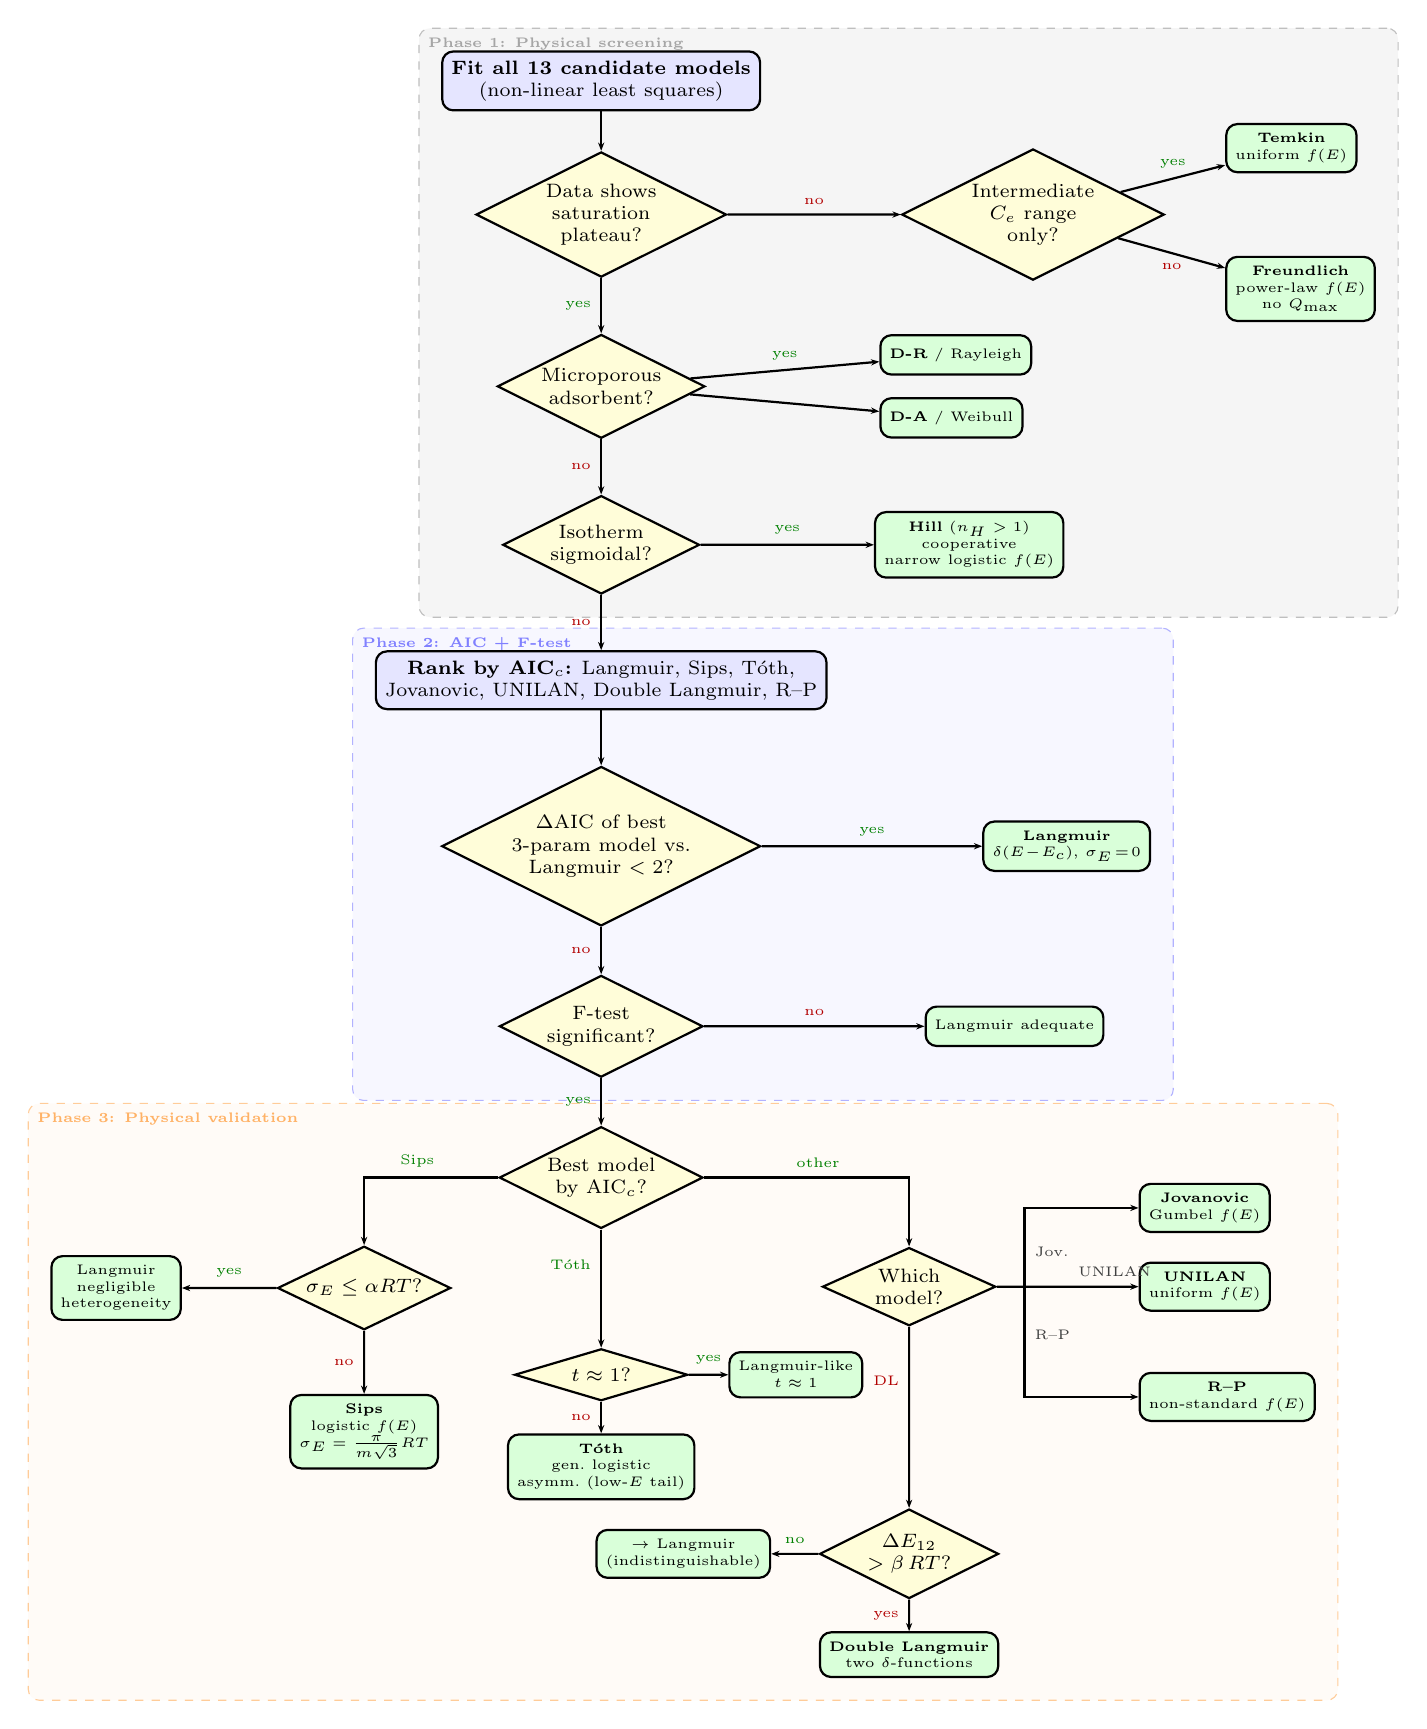
\begin{tikzpicture}[
		scale=0.78, every node/.append style={transform shape},
		every node/.style={font=\scriptsize},
		decision/.style={draw, diamond, aspect=2, inner sep=1pt,
			minimum width=2.2cm, align=center, thick, fill=yellow!15},
		result/.style={draw, rounded corners, minimum width=1.6cm,
			minimum height=0.5cm, align=center, thick, fill=green!15,
			font=\tiny},
		process/.style={draw, rounded corners, minimum width=2.2cm,
			minimum height=0.5cm, align=center, thick, fill=blue!10},
		arr/.style={-{Stealth[length=3pt]}, thick},
		yeslbl/.style={font=\tiny, green!50!black},
		nolbl/.style={font=\tiny, red!70!black},
		choicelbl/.style={font=\tiny, black!75},
		]

		% ============ PHASE 1: Physical screening ============
		\node[process] (fit) {\textbf{Fit all 13 candidate models}\\
			(non-linear least squares)};

		% --- Q1: saturation ---
		\node[decision, below=0.5cm of fit] (q1)
		{Data shows\\saturation\\plateau?};

		% NO saturation branch (right)
		\node[decision, right=2.2cm of q1] (q1b)
		{Intermediate\\$C_e$ range\\only?};
		\node[result, above right=0.1cm and 1.6cm of q1b] (r_temkin)
		{\textbf{Temkin}\\uniform $f(E)$};
		\node[result, below right=0.1cm and 1.6cm of q1b] (r_freund)
		{\textbf{Freundlich}\\power-law $f(E)$\\no $Q_{\max}$};

		% YES saturation branch (down)
		\node[decision, below=0.7cm of q1] (q2)
		{Microporous\\adsorbent?};

		% DR/DA branch (right)
		\node[result, right=2.2cm of q2, yshift=0.4cm] (r_DR)
		{\textbf{D-R} / Rayleigh};
		\node[result, right=2.2cm of q2, yshift=-0.4cm] (r_DA)
		{\textbf{D-A} / Weibull};

		% Continue down
		\node[decision, below=0.7cm of q2] (q3)
		{Isotherm\\sigmoidal?};

		% Hill branch (right)
		\node[result, right=2.2cm of q3] (r_hill)
		{\textbf{Hill} ($n_H > 1$)\\cooperative\\narrow logistic $f(E)$};

		% AIC ranking
		\node[process, below=0.7cm of q3] (aic)
		{\textbf{Rank by AIC$_c$:} Langmuir, Sips, T\'{o}th,\\
			Jovanovic, UNILAN, Double Langmuir, R--P};

		% ============ PHASE 2: AIC + F-test ============
		\node[decision, below=0.7cm of aic] (d1)
		{$\Delta\mathrm{AIC}$ of best\\3-param model vs.\\ Langmuir $< 2$?};
		\node[result, right=2.8cm of d1] (r_lang)
		{\textbf{Langmuir}\\$\delta(E\!-\!E_c)$, $\sigma_E\!=\!0$};

		\node[decision, below=0.6cm of d1] (d2)
		{F-test\\significant?};
		\node[result, right=2.8cm of d2] (r_lang2)
		{Langmuir adequate};

		% ============ PHASE 3: Which heterogeneous model? ============
		\node[decision, below=0.6cm of d2] (d3)
		{Best model\\by AIC$_c$?};

		% --- Left column: Sips ---
		\node[decision, below left=0.8cm and 1.8cm of d3] (d_sips)
		{$\sigma_E \leq \alpha RT$?};
		\node[result, left=1.2cm of d_sips ] (r_sips_neg)
		{Langmuir\\negligible\\heterogeneity};
		\node[result, below=0.8cm of d_sips] (r_sips)
		{\textbf{Sips}\\logistic $f(E)$\\
			$\sigma_E = \frac{\pi}{m\sqrt{3}}RT$};

		% --- Center column: Toth ---
		\node[decision, below=1.5cm of d3] (d_toth)
		{$t \approx 1$?};
		\node[result, right=0.5cm of d_toth] (r_toth_yes)
		{Langmuir-like\\$t \approx 1$};
		\node[result, below=0.4cm of d_toth] (r_toth)
		{\textbf{T\'{o}th}\\gen.\ logistic\\asymm.\ (low-$E$ tail)};

		% --- Right column: Jov / UNILAN / RP / DL ---
		\node[decision, below right=0.8cm and 2.7cm of d3] (d_right)
		{Which\\model?};

		% Terminal results stacked vertically on the right
		\node[result, right=1.8cm of d_right, yshift=1.0cm] (r_jov)
		{\textbf{Jovanovic}\\Gumbel $f(E)$};
		\node[result, right=1.8cm of d_right, yshift=-0.0cm] (r_unilan)
		{\textbf{UNILAN}\\uniform $f(E)$};
		\node[result, right=1.8cm of d_right, yshift=-1.4cm] (r_RP)
		{\textbf{R--P}\\non-standard $f(E)$};

		% Double Langmuir sub-decision
		\node[decision, below=2.3cm of d_right] (d_DL)
		{$\Delta E_{12}$\\$> \beta\,RT$?};
		\node[result, below=0.4cm of d_DL] (r_DL)
		{\textbf{Double Langmuir}\\two $\delta$-functions};
		\node[result, left=0.6cm of d_DL] (r_DL_no)
		{$\to$ Langmuir\\(indistinguishable)};

		% ============ ARROWS ============
		% Phase 1
		\draw[arr] (fit) -- (q1);
		\draw[arr] (q1) -- node[nolbl, above] {no} (q1b);
		\draw[arr] (q1b) -- node[yeslbl, above] {yes} (r_temkin);
		\draw[arr] (q1b) -- node[nolbl, below] {no} (r_freund);
		\draw[arr] (q1) -- node[yeslbl, left] {yes} (q2);
		\draw[arr] (q2) -- node[yeslbl, above] {yes} (r_DR);
		\draw[arr] (q2) -- node[yeslbl, below] {} (r_DA);
		\draw[arr] (q2) -- node[nolbl, left] {no} (q3);
		\draw[arr] (q3) -- node[yeslbl, above] {yes} (r_hill);
		\draw[arr] (q3) -- node[nolbl, left] {no} (aic);

		% Phase 2
		\draw[arr] (aic) -- (d1);
		\draw[arr] (d1) -- node[yeslbl, above] {yes} (r_lang);
		\draw[arr] (d1) -- node[nolbl, left] {no} (d2);
		\draw[arr] (d2) -- node[nolbl, above] {no} (r_lang2);
		\draw[arr] (d2) -- node[yeslbl, left] {yes} (d3);

		% Phase 3: branching from d3
		\draw[arr] (d3) -| node[yeslbl, above left, pos=0.2]
		{Sips} (d_sips);
		\draw[arr] (d3) -- node[yeslbl, left, pos=0.3]
		{T\'{o}th} (d_toth);
		\draw[arr] (d3) -| node[yeslbl, above right, pos=0.2]
		{other} (d_right);

		% Sips sub-tree
		\draw[arr] (d_sips) -- node[yeslbl, above] {yes} (r_sips_neg);
		\draw[arr] (d_sips) -- node[nolbl, left] {no} (r_sips);

		% Toth sub-tree
		\draw[arr] (d_toth) -- node[nolbl, left] {no} (r_toth);
		\draw[arr] (d_toth) -- node[yeslbl, above] {yes} (r_toth_yes);

		% Right sub-tree
		\draw[arr] (d_right.east) -- ++(0.45,0)
		|- node[choicelbl, pos=0.22, right] {Jov.} (r_jov.west);
		\draw[arr] (d_right.east) -- ++(0.75,0)
		-- node[choicelbl, above, pos=0.75] {UNILAN} (r_unilan.west);
		\draw[arr] (d_right.east) -- ++(0.45,0)
		|- node[choicelbl, pos=0.22, right] {R--P} (r_RP.west);
		\draw[arr] (d_right) -- node[nolbl, left, pos=0.3] {DL} (d_DL);
		\draw[arr] (d_DL) -- node[nolbl, left] {yes} (r_DL);
		\draw[arr] (d_DL) -- node[yeslbl, above] {no} (r_DL_no);

		% ============ Phase background boxes ============
		\begin{scope}[on background layer]
			\node[draw=gray!50, dashed, fill=gray!8,
			rounded corners=4pt, inner sep=8pt,
			fit=(fit)(q1)(q3)(r_hill)(r_temkin)(r_freund)(r_DR)(r_DA),
			label={[font=\tiny\bfseries, gray!70, anchor=north west]
				north west:Phase 1: Physical screening}] {};
			\node[draw=blue!30, dashed, fill=blue!3,
			rounded corners=4pt, inner sep=8pt,
			fit=(aic)(d1)(d2)(r_lang)(r_lang2),
			label={[font=\tiny\bfseries, blue!50, anchor=north west]
				north west:Phase 2: AIC + F-test}] {};
			\node[draw=orange!40, dashed, fill=orange!3,
			rounded corners=4pt, inner sep=8pt,
			fit=(d3)(d_sips)(d_toth)(d_right)(d_DL)
			(r_sips)(r_sips_neg)(r_toth)(r_toth_yes)(r_jov)(r_unilan)(r_RP)
			(r_DL)(r_DL_no),
			label={[font=\tiny\bfseries, orange!60, anchor=north west]
				north west:Phase 3: Physical validation}] {};
		\end{scope}
	\end{tikzpicture}
	\caption{Complete decision tree for isotherm model selection.
		\textbf{Phase~1} (top): physical screening based on data shape
		--- saturation plateau, micropore filling, sigmoidal curvature.
		\textbf{Phase~2} (middle): AIC$_c$ ranking and F-test for all
		saturating models.
		\textbf{Phase~3} (bottom): pairwise tests combined with physical
		criteria ($\sigma_E$, $\Delta E_{12}$, $t$, $\beta$).
		Green terminal boxes show the accepted model and its
		energy-distribution family.}
	\label{fig:si_decision_tree}
\end{figure}


% =====================================================================
%  SECTION S-5: ENERGY DISTRIBUTIONS
% =====================================================================
\section{Energy distributions of adsorption isotherms}
\label{sec:si_distributions}

\subsection{General framework}
\label{sec:si_energy_framework}

A heterogeneous surface is described as a collection of independent
Langmuir sites, each with adsorption energy~$E$.  The macroscopic
isotherm is the integral:
\begin{equation}
	q_e = Q_{\max} \int_{0}^{\infty}
	\frac{K(E)\, C_e}{1 + K(E)\, C_e}\, f(E)\, \mathrm{d}E,
	\label{eq:si_heterogeneous_integral}
\end{equation}
where $K(E) = K_0\exp(E/RT)$ and $f(E)$ is the normalised site-energy
distribution.  Different choices of $f(E)$ yield different
macroscopic isotherms.

In the \emph{condensation approximation}, the substitution
\begin{equation}
	C_e = C^{\ast}\exp(-E/RT)
	\label{eq:si_condensation}
\end{equation}
maps the isotherm $q(C_e)$ into $q(E)$, and the energy distribution
is recovered by differentiation:
\begin{equation}
	f(E) = -\frac{\mathrm{d}q}{\mathrm{d}E}.
	\label{eq:si_fE_derivative}
\end{equation}

\subsection{Summary of all energy distributions}
\label{sec:si_dist_summary}

Table~\ref{tab:si_energy_dist_families} collects the distribution
family, symmetry, and width parameter $\sigma_E$ for every isotherm
model.

\begin{table}[H]
	\centering
	\small
	\caption{Energy-distribution families implied by each isotherm model.
		All distributions are expressed in the reduced energy
		$u = (E - E_c)/(RT)$.  The standard deviation $\sigma_E$ is given
		in units of $RT$ ($\approx 2.478$~kJ/mol at $T = 298$~K).}
	\label{tab:si_energy_dist_families}
	\renewcommand{\arraystretch}{1.5}
	\begin{tabular}{@{} l l c c l @{}}
		\toprule
		\textbf{Model}
		& \textbf{Distribution $f(E)$}
		& \textbf{Symmetry}
		& $\boldsymbol{\sigma_E/(RT)}$
		& \textbf{Fit parameters} \\
		\midrule
		Langmuir
		& Dirac $\delta(E - E_c)$
		& ---
		& $0$
		& $K_L,\, Q_{\max}$ \\
		%
		Double Langmuir
		& Two Dirac $\delta$
		& ---
		& $\dfrac{\sqrt{Q_1Q_2}}{Q_1+Q_2}\dfrac{|\Delta E_{12}|}{RT}$
		& $K_1, K_2, Q_1, Q_2$ \\
		%
		Sips (L--F)
		& Logistic
		& Symmetric
		& $\pi/(m\sqrt{3})$
		& $K_S,\, m,\, Q_{\max}$ \\
		%
		T\'{o}th
		& Gen.\ logistic (IV)
		& Asymmetric
		& $> \pi/\sqrt{3}$\;($t<1$)
		& $b,\, t,\, q_{\max}$ \\
		%
		Jovanovic
		& Gumbel (EV-I)
		& Asymmetric
		& $\pi/\sqrt{6} \approx 1.28$
		& $b,\, q_{\max}$ \\
		%
		Temkin
		& Uniform (rect.)
		& Symmetric
		& $\dfrac{b_T Q_{\max}}{2\sqrt{3}\,RT}$
		& $a_T,\, b_T$ \\
		%
		UNILAN
		& Uniform (rect.)
		& Symmetric
		& $\dfrac{\ln(b_{\max}/b_{\min})}{2\sqrt{3}}$
		& $b_{\max}, b_{\min}, q_{\max}$ \\
		%
		Freundlich
		& Power law
		& ---
		& $\infty$
		& $K_F,\, 1/n$ \\
		%
		Redlich--Peterson
		& Non-standard
		& Asymm.\ ($\beta<1$)
		& ---
		& $K_{RP}, a_{RP}, \beta$ \\
		%
		Koble--Corrigan
		& $\equiv$ Sips
		& Symmetric
		& $\pi n/\sqrt{3}$
		& $A_{KC}, B_{KC}, 1/n$ \\
		%
		Radke--Prausnitz
		& Non-standard
		& Asymmetric
		& ---
		& $a_{RP}, r_{RP}, p$ \\
		%
		D-R
		& Rayleigh
		& Asymmetric
		& $0.463\,E_a/RT$
		& $Q_{\max},\, E_a$ \\
		%
		D-A
		& Weibull
		& Asymmetric
		& $\frac{E_a}{RT}\!\sqrt{\Gamma(1\!+\!\frac{2}{n})\!-\!\Gamma(1\!+\!\frac{1}{n})^2}$
		& $Q_{\max}, E_a, n_{DA}$ \\
		%
		Hill
		& $\equiv$ Sips
		& Symmetric
		& $\pi/(\sqrt{3}\,n_H)$
		& $Q_{\max}, K_D, n_H$ \\
		\bottomrule
	\end{tabular}
\end{table}

\subsection{Numerical values of $\sigma_E$ at $T = 298$~K}
\label{sec:si_sigma_numerical}

Table~\ref{tab:si_sigma_numerical} gives numerical values of $\sigma_E$
for representative parameter choices at $T = 298$~K
($RT = 2.478$~kJ\,mol$^{-1}$).

\begin{table}[H]
	\centering
	\small
	\caption{Numerical values of $\sigma_E$ at $T = 298$~K
		($RT = 2.478$~kJ\,mol$^{-1}$) for representative parameter values.}
	\label{tab:si_sigma_numerical}
	\renewcommand{\arraystretch}{1.3}
	\begin{tabular}{@{} l l c c @{}}
		\toprule
		\textbf{Model} & \textbf{Parameter}
		& $\boldsymbol{\sigma_E/(RT)}$
		& $\boldsymbol{\sigma_E}$ (kJ/mol) \\
		\midrule
		Sips & $n = 1.0$ & 1.81 & 4.49 \\
		Sips & $n = 1.5$ & 2.72 & 6.74 \\
		Sips & $n = 2.0$ & 3.63 & 8.99 \\
		Sips & $n = 3.0$ & 5.44 & 13.48 \\
		\midrule
		T\'{o}th & $t = 0.7$ & 2.17 & 5.38 \\
		T\'{o}th & $t = 0.5$ & 2.65 & 6.56 \\
		T\'{o}th & $t = 0.3$ & 3.51 & 8.70 \\
		\midrule
		Jovanovic & --- & 1.28 & 3.18 \\
		\midrule
		Temkin/UNILAN & $s = 2\,RT$ & 1.15 & 2.86 \\
		Temkin/UNILAN & $s = 3\,RT$ & 1.73 & 4.29 \\
		Temkin/UNILAN & $s = 4\,RT$ & 2.31 & 5.72 \\
		\midrule
		Hill & $n_H = 0.5$ & 3.63 & 8.99 \\
		Hill & $n_H = 1.0$ & 1.81 & 4.49 \\
		Hill & $n_H = 2.0$ & 0.91 & 2.24 \\
		Hill & $n_H = 4.0$ & 0.45 & 1.12 \\
		\midrule
		D-R & $E_a = 10$ kJ/mol & 1.87 & 4.63 \\
		D-R & $E_a = 20$ kJ/mol & 3.74 & 9.27 \\
		\bottomrule
	\end{tabular}
\end{table}

\subsection{Individual energy distributions and $\sigma_E$ derivations}
\label{sec:si_individual_distributions}

The condensation approximation (Section~\ref{sec:si_energy_framework}) is applied
to each isotherm by substituting $C_e = C^{\ast}\mathrm{e}^{-E/RT}$ and computing
$f(E) = -(1/Q_{\max})\,\mathrm{d}q/\mathrm{d}E$. The standard deviation $\sigma_E$
is then obtained from the variance of the resulting distribution family.

% ------ Langmuir ------
\subsubsection{Langmuir}

\paragraph{Exact result.}
The Langmuir isotherm is obtained \emph{exactly} by setting
$f(E) = \delta(E-E_c)$ in Eq.~\eqref{eq:si_heterogeneous_integral}:
\begin{equation}
	Q_{\max}\int_0^{\infty}\frac{K(E)\,C_e}{1+K(E)\,C_e}
	\,\delta(E-E_c)\,\mathrm{d}E
	= Q_{\max}\,\frac{K_L\,C_e}{1+K_L\,C_e},
	\qquad K_L = K_0\mathrm{e}^{E_c/RT}.
\end{equation}
No condensation approximation is needed: the Langmuir isotherm is \emph{exact}
for a homogeneous surface ($\sigma_E = 0$).

\paragraph{Characteristic energy and width.}
\begin{equation}
	E_c = RT\ln(K_L\,C^{\ast}), \qquad \sigma_E = 0.
\end{equation}

% ------ Double Langmuir ------
\subsubsection{Double Langmuir}

\paragraph{Distribution.}
The double-Langmuir isotherm follows from a bimodal discrete distribution:
\begin{equation}
	f(E) = \frac{Q_1}{Q_{\max}}\,\delta(E-E_1)
	     + \frac{Q_2}{Q_{\max}}\,\delta(E-E_2),
	\qquad Q_{\max} = Q_1+Q_2,
\end{equation}
with $E_i = RT\ln(K_i\,C^{\ast})$.

\paragraph{Derivation of $\sigma_E$.}
For a two-point distribution with weights $w_i = Q_i/Q_{\max}$:
\begin{align}
	\langle E \rangle &= w_1 E_1 + w_2 E_2, \\
	\sigma_E^2 &= w_1(E_1-\langle E\rangle)^2 + w_2(E_2-\langle E\rangle)^2
	           = w_1 w_2\,(E_1-E_2)^2,
\end{align}
therefore
\begin{equation}
	\sigma_E = \frac{\sqrt{Q_1 Q_2}}{Q_1+Q_2}\,|\Delta E_{12}|,
	\qquad \Delta E_{12} = E_1 - E_2.
	\label{eq:si_sigmaE_DL}
\end{equation}
For equal sites ($Q_1=Q_2$): $\sigma_E = |\Delta E_{12}|/2$.

% ------ Sips ------
\subsubsection{Sips (Langmuir--Freundlich)}
\label{sec:si_sips_dist}

\paragraph{Starting isotherm.}
\begin{equation}
	q_e = Q_{\max}\,\frac{K_S C_e^{m}}{1 + K_S C_e^{m}},
	\qquad 0 < m \leq 1.
\end{equation}

\paragraph{Condensation substitution.}
Setting $C_e = C^{\ast}\mathrm{e}^{-E/RT}$ and defining
$E_c = (RT/m)\ln[K_S(C^{\ast})^{m}] = RT\ln(K_S^{1/m}C^{\ast})$:
\begin{equation}
	q(E) = \frac{Q_{\max}}{1+\mathrm{e}^{m(E-E_c)/RT}}.
\end{equation}

\paragraph{Differentiation.}
\begin{equation}
	\frac{\mathrm{d}q}{\mathrm{d}E}
	= -Q_{\max}\,\frac{(m/RT)\,\mathrm{e}^{m(E-E_c)/RT}}
	           {\bigl[1+\mathrm{e}^{m(E-E_c)/RT}\bigr]^{2}}.
\end{equation}

\paragraph{Distribution.}
\begin{equation}
	f(E) = \frac{Q_{\max}\,(m/RT)\,\mathrm{e}^{m(E-E_c)/RT}}
	           {\bigl[1+\mathrm{e}^{m(E-E_c)/RT}\bigr]^{2}}.
	\label{eq:si_fE_sips}
\end{equation}
This is the \textbf{logistic} probability density (times $Q_{\max}$)
with location $E_c$ and scale $s = RT/m$.

\paragraph{Width.}
The variance of the logistic distribution with scale $s$ is $\pi^2 s^2/3$, so
\begin{equation}
	\sigma_E = \frac{\pi}{\sqrt{3}}\,\frac{RT}{m}.
	\label{eq:si_sigmaE_sips}
\end{equation}
For $m=1$ (Langmuir): $\sigma_E = (\pi/\sqrt{3})\,RT \approx 1.81\,RT$.
As $m \to 0$: $\sigma_E \to \infty$ (Freundlich limit).

% ------ Toth ------
\subsubsection{T\'{o}th}

\paragraph{Starting isotherm.}
\begin{equation}
	q_e = \frac{q_{\max}\, b\, C_e}{\bigl[1+(b C_e)^{t}\bigr]^{1/t}},
	\qquad 0 < t \leq 1.
\end{equation}

\paragraph{Condensation substitution.}
Setting $C_e = C^{\ast}\mathrm{e}^{-E/RT}$, $E_c = RT\ln(bC^{\ast})$,
$u = (E-E_c)/RT$:
\begin{equation}
	q(E) = q_{\max}\,\frac{\mathrm{e}^{-u}}{\bigl[1+\mathrm{e}^{-tu}\bigr]^{1/t}}.
\end{equation}

\paragraph{Differentiation.}
Applying the product rule and collecting terms:
\begin{equation}
	\frac{\mathrm{d}q}{\mathrm{d}E}
	= -\frac{q_{\max}}{RT}\,\frac{\mathrm{e}^{-u}}
	                               {\bigl[1+\mathrm{e}^{-tu}\bigr]^{(1+t)/t}},
	\qquad u = \frac{E-E_c}{RT}.
\end{equation}

\paragraph{Distribution.}
\begin{equation}
	f(E) = \frac{q_{\max}}{RT}\,
	\frac{\mathrm{e}^{-u}}
	{[1 + \mathrm{e}^{-tu}]^{(1+t)/t}},
	\qquad u = \frac{E - E_c}{RT}.
	\label{eq:si_fE_toth}
\end{equation}
This is the \textbf{generalised logistic type IV}, asymmetric with a heavier tail
toward \emph{low} adsorption energies for $t < 1$.
For $t = 1$ it reduces to the standard logistic (Langmuir limit).

\paragraph{Width.}
No closed-form $\sigma_E$ exists for general $t$; numerical integration is required.
$\sigma_E > (\pi/\sqrt{3})\,RT$ for all $t < 1$, diverging as $t \to 0$.

% ------ Jovanovic ------
\subsubsection{Jovanovic}

\paragraph{Starting isotherm.}
\begin{equation}
	q_e = q_{\max}\bigl[1 - \exp(-b C_e)\bigr].
\end{equation}

\paragraph{Condensation substitution.}
Setting $C_e = C^{\ast}\mathrm{e}^{-E/RT}$, $E_c = RT\ln(bC^{\ast})$,
$u = (E-E_c)/RT$:
\begin{equation}
	q(E) = q_{\max}\!\left[1 - \exp\!\left(-\mathrm{e}^{-u}\right)\right].
\end{equation}

\paragraph{Differentiation.}
\begin{equation}
	\frac{\mathrm{d}q}{\mathrm{d}E}
	= -\frac{q_{\max}}{RT}\,\mathrm{e}^{-u}\exp\!\left(-\mathrm{e}^{-u}\right).
\end{equation}

\paragraph{Distribution.}
\begin{equation}
	f(E) = \frac{q_{\max}}{RT}\,\mathrm{e}^{-u}\exp\!\left(-\mathrm{e}^{-u}\right),
	\qquad u = \frac{E-E_c}{RT}.
	\label{eq:si_fE_jov}
\end{equation}
This is the \textbf{Gumbel (extreme-value type I)} distribution with location $E_c$
and scale $RT$. The mean is $\langle E\rangle = E_c + \gamma\,RT$
($\gamma \approx 0.5772$, Euler--Mascheroni constant).
The distribution is asymmetric with a longer tail toward \emph{high} energies.

\paragraph{Width.}
The variance of the Gumbel distribution with scale $\beta$ is $\pi^2\beta^2/6$:
\begin{equation}
	E_c = RT\ln(bC^{\ast}),
	\qquad
	\sigma_E = \frac{\pi}{\sqrt{6}}\,RT \approx 1.283\,RT.
	\label{eq:si_sigmaE_jov}
\end{equation}
The width is independent of the affinity parameter $b$ and is fixed solely by
the model functional form.

% ------ Temkin ------
\subsubsection{Temkin}

\paragraph{Starting isotherm.}
\begin{equation}
	q_e = \frac{RT}{b_T}\ln(a_T C_e).
\end{equation}
(Valid over the intermediate concentration range where the log-linear
approximation holds; implicitly defines $[E_{\min}, E_{\max}]$.)

\paragraph{Condensation substitution.}
Setting $C_e = C^{\ast}\mathrm{e}^{-E/RT}$:
\begin{equation}
	q(E) = \frac{1}{b_T}\bigl[RT\ln(a_T C^{\ast}) - E\bigr].
\end{equation}

\paragraph{Distribution.}
\begin{equation}
	f(E) = -\frac{1}{Q_{\max}}\frac{\mathrm{d}q}{\mathrm{d}E}
	= \frac{Q_{\max}}{b_T Q_{\max}} = \frac{1}{b_T} = \text{const},
	\qquad E_{\min} \leq E \leq E_{\max}.
	\label{eq:si_fE_temkin}
\end{equation}
This is a \textbf{uniform (rectangular)} distribution over $[E_{\min}, E_{\max}]$,
where $E_{\max} = RT\ln(a_T C^{\ast})$ and $E_{\max} - E_{\min} = b_T Q_{\max}$.

\paragraph{Width.}
For a uniform distribution on $[a,b]$, $\sigma = (b-a)/(2\sqrt{3})$:
\begin{equation}
	\sigma_E = \frac{E_{\max}-E_{\min}}{2\sqrt{3}}
	= \frac{b_T\,Q_{\max}}{2\sqrt{3}}.
	\label{eq:si_sigmaE_temkin}
\end{equation}

% ------ UNILAN ------
\subsubsection{UNILAN}

\paragraph{Exact integration.}
UNILAN retains the full Langmuir kernel and integrates over a uniform distribution
$f(E) = Q_{\max}/(2s)$ on $[E_c-s,\,E_c+s]$ analytically:
\begin{align}
	q_e &= \frac{Q_{\max}}{2s}\int_{E_c-s}^{E_c+s}
	\frac{K_0\mathrm{e}^{E/RT}\,C_e}{1+K_0\mathrm{e}^{E/RT}\,C_e}\,\mathrm{d}E
	\notag \\
	&= \frac{Q_{\max}\,RT}{2s}
	\ln\!\frac{1+b_{\max}\,C_e}{1+b_{\min}\,C_e},
	\qquad b_{\max/\min} = K_0\,\mathrm{e}^{(E_c\pm s)/RT}.
\end{align}

\paragraph{Distribution and width.}
By construction:
\begin{equation}
	f(E) = \frac{Q_{\max}}{2s} = \text{const},
	\qquad s = \frac{RT}{2}\ln\!\frac{b_{\max}}{b_{\min}}.
	\label{eq:si_fE_unilan}
\end{equation}
The standard deviation of the uniform distribution on $[E_c-s,\,E_c+s]$ is $s/\sqrt{3}$:
\begin{equation}
	\sigma_E = \frac{s}{\sqrt{3}}
	= \frac{RT}{2\sqrt{3}}\ln\!\frac{b_{\max}}{b_{\min}}.
	\label{eq:si_sigmaE_unilan}
\end{equation}

% ------ Freundlich ------
\subsubsection{Freundlich}

\paragraph{Starting isotherm.}
\begin{equation}
	q_e = K_F C_e^{1/n}, \qquad 0 < 1/n < 1.
\end{equation}

\paragraph{Condensation substitution.}
Setting $C_e = C^{\ast}\mathrm{e}^{-E/RT}$:
\begin{equation}
	q(E) = K_F(C^{\ast})^{1/n}\,\mathrm{e}^{-E/(nRT)}.
\end{equation}

\paragraph{Distribution.}
\begin{equation}
	f(E) = \frac{K_F(C^{\ast})^{1/n}}{nRT}\,\mathrm{e}^{-E/(nRT)}.
	\label{eq:si_fE_freundlich}
\end{equation}
This one-sided exponential does \emph{not} normalise to a finite area on
$[0,\infty)$, reflecting the absence of a finite $Q_{\max}$.

\paragraph{Width.}
$\sigma_E = \infty$. The Freundlich model cannot be interpreted as arising from
a physically normalised site-energy distribution; it is a purely empirical
fitting equation valid only over a limited concentration window.

% ------ Redlich-Peterson ------
\subsubsection{Redlich--Peterson}

\paragraph{Starting isotherm.}
\begin{equation}
	q_e = \frac{K_{RP}\,C_e}{1 + a_{RP}\,C_e^{\beta}},
	\qquad 0 < \beta \leq 1.
\end{equation}

\paragraph{Condensation substitution and distribution.}
Setting $C_e = C^{\ast}\mathrm{e}^{-E/RT}$ and differentiating:
\begin{equation}
	f(E) = \frac{K_{RP}\,C^{\ast}\mathrm{e}^{-E/RT}}{Q_{\max}\,RT}
	\cdot\frac{1+(1-\beta)\,a_{RP}(C^{\ast})^{\beta}\mathrm{e}^{-\beta E/RT}}
	          {\bigl[1+a_{RP}(C^{\ast})^{\beta}\mathrm{e}^{-\beta E/RT}\bigr]^{2}}.
	\label{eq:si_fE_RP}
\end{equation}
For $\beta = 1$: reduces to the logistic density (Langmuir). For $\beta < 1$:
non-standard asymmetric form with no closed-form $\sigma_E$.

% ------ Koble-Corrigan ------
\subsubsection{Koble--Corrigan}

\paragraph{Equivalence to Sips.}
The Koble--Corrigan isotherm
$q_e = A_{KC}\,C_e^{m}\,/\,(1 + B_{KC}\,C_e^{m})$
is algebraically identical to Sips with $Q_{\max} = A_{KC}/B_{KC}$ and
$K_S = B_{KC}$, same exponent $m$.
The energy distribution and $\sigma_E$ are therefore those of
Section~\ref{sec:si_sips_dist}:
\begin{equation}
	\sigma_E = \frac{\pi}{\sqrt{3}}\,\frac{RT}{m}.
\end{equation}

% ------ Radke-Prausnitz ------
\subsubsection{Radke--Prausnitz}

\paragraph{Starting isotherm.}
\begin{equation}
	q_e = \frac{a_{RP}\,r_{RP}\,C_e}{a_{RP} + r_{RP}\,C_e^{p}},
	\qquad 0 < p \leq 1.
\end{equation}

\paragraph{Distribution.}
Applying the condensation substitution yields a non-standard distribution
without a simple closed form. No analytical $\sigma_E$ exists; numerical
integration is required. For $p \to 0$ the distribution approaches a
logarithmic form with diverging width; for $p = 1$ it reduces to the
Langmuir (logistic) distribution.

% ------ D-R / D-A ------
\subsubsection{Dubinin--Radushkevich / Dubinin--Astakhov}

\paragraph{Polanyi potential.}
D-R and D-A operate in the Polanyi adsorption potential
$\varepsilon = RT\ln(1 + 1/C_e)$ rather than directly in $E$.
The isotherm is
\begin{equation}
	q_e = Q_{\max}\exp\!\left[-\!\left(\frac{\varepsilon}{E_a}\right)^{\!n_{DA}}\right].
\end{equation}

\paragraph{Derivation of $f(\varepsilon)$.}
Differentiating with respect to $\varepsilon$:
\begin{equation}
	f(\varepsilon) = -\frac{1}{Q_{\max}}\frac{\mathrm{d}q}{\mathrm{d}\varepsilon}
	= \frac{n_{DA}}{E_a}\left(\frac{\varepsilon}{E_a}\right)^{n_{DA}-1}
	\exp\!\left[-\!\left(\frac{\varepsilon}{E_a}\right)^{n_{DA}}\right].
	\label{eq:si_fE_DA}
\end{equation}
This is the \textbf{Weibull} probability density with scale $E_a$
and shape $n_{DA}$.

\paragraph{Mean adsorption potential.}
\begin{equation}
	\langle\varepsilon\rangle
	= \frac{E_a}{n_{DA}}\,\Gamma\!\left(\frac{1}{n_{DA}}\right).
\end{equation}
D-R ($n_{DA}=2$): $\langle\varepsilon\rangle = E_a\sqrt{\pi}/2$.

\paragraph{Width.}
The variance of the Weibull distribution with scale $E_a$ and shape $n_{DA}$ is
$E_a^2[\Gamma(1+2/n_{DA})-\Gamma(1+1/n_{DA})^2]$, therefore
\begin{equation}
	\sigma_\varepsilon
	= E_a\sqrt{\Gamma\!\left(1+\frac{2}{n_{DA}}\right)
	           - \left[\Gamma\!\left(1+\frac{1}{n_{DA}}\right)\right]^{2}}.
	\label{eq:si_sigmaE_DA}
\end{equation}
D-R ($n_{DA}=2$): $\Gamma(2)=1$, $\Gamma(3/2)=\sqrt{\pi}/2$, so
\begin{equation}
	\sigma_\varepsilon = E_a\sqrt{1-\pi/4} \approx 0.4633\,E_a.
\end{equation}
The distribution is right-skewed (longer tail toward high adsorption potentials).

% ------ Hill ------
\subsubsection{Hill}

\paragraph{Starting isotherm.}
\begin{equation}
	q_e = \frac{Q_{\max}\,C_e^{n_H}}{K_D + C_e^{n_H}}.
\end{equation}

\paragraph{Condensation substitution.}
Setting $C_e = C^{\ast}\mathrm{e}^{-E/RT}$ and defining
$E_c = RT\ln(K_D^{-1/n_H}\,C^{\ast})$:
\begin{equation}
	q(E) = \frac{Q_{\max}}{1+\mathrm{e}^{n_H(E-E_c)/RT}}.
\end{equation}

\paragraph{Differentiation.}
\begin{equation}
	\frac{\mathrm{d}q}{\mathrm{d}E}
	= -Q_{\max}\,\frac{(n_H/RT)\,\mathrm{e}^{n_H(E-E_c)/RT}}
	           {\bigl[1+\mathrm{e}^{n_H(E-E_c)/RT}\bigr]^{2}}.
\end{equation}

\paragraph{Distribution.}
\begin{equation}
	f(E) = \frac{Q_{\max}\,(n_H/RT)\,\mathrm{e}^{n_H(E-E_c)/RT}}
	           {\bigl[1+\mathrm{e}^{n_H(E-E_c)/RT}\bigr]^{2}}.
	\label{eq:si_fE_Hill}
\end{equation}
Logistic density (times $Q_{\max}$) with location $E_c$ and scale $s = RT/n_H$;
identical in form to Sips (Section~\ref{sec:si_sips_dist}) with $m \to n_H$.

\paragraph{Width.}
\begin{equation}
	E_c = RT\ln(K_D^{-1/n_H}\,C^{\ast}),
	\qquad
	\sigma_E = \frac{\pi}{\sqrt{3}}\,\frac{RT}{n_H}.
	\label{eq:si_sigmaE_Hill}
\end{equation}

\paragraph{Physical interpretation.}
\begin{itemize}
	\item $n_H < 1$ (anti-cooperative): $\sigma_E > (\pi/\sqrt{3})\,RT$ --- broader than Langmuir.
	\item $n_H = 1$ (non-cooperative): $\sigma_E = (\pi/\sqrt{3})\,RT \approx 1.81\,RT$.
	\item $n_H > 1$ (cooperative binding): $\sigma_E < (\pi/\sqrt{3})\,RT$ ---
	      narrower distribution; the adsorption transition is sharper.
\end{itemize}

\begin{comment}
	

\subsection{Visualisation of energy distributions}
\label{sec:si_energy_visualisation}

Figures~\ref{fig:si_energy_overview}, \ref{fig:si_energy_panels},
and~\ref{fig:si_sigma_vs_het} show the normalised energy distributions
generated by the companion MATLAB script
\texttt{plot\_energy\_distributions.m}.

\begin{figure}[H]
	\centering
	\includegraphics[width=0.85\linewidth]{fig_energy_distributions.pdf}
	\caption{Comparative overlay of normalised site-energy distributions
		$\phi(u) = f(E)/Q_{\max}$ for representative isotherm models,
		plotted in reduced energy $u = (E - E_c)/(RT)$.}
	\label{fig:si_energy_overview}
\end{figure}

\begin{figure}[H]
	\centering
	\includegraphics[width=\linewidth]{fig_energy_distributions_panel.pdf}
	\caption{Individual energy-distribution families with parameter
		variations: (a)~Sips, (b)~T\'{o}th, (c)~Jovanovic,
		(d)~Temkin/UNILAN, (e)~Freundlich, (f)~D-R/D-A (Weibull),
		(g)~Hill, (h)~Redlich--Peterson, (i)~Langmuir.}
	\label{fig:si_energy_panels}
\end{figure}

\begin{figure}[H]
	\centering
	\includegraphics[width=0.75\linewidth]{fig_sigma_vs_heterogeneity.pdf}
	\caption{Energy-distribution width $\sigma_E/(RT)$ as a function
		of the heterogeneity parameter for Sips and Hill isotherms.
		The Jovanovic value ($\pi/\sqrt{6}$) is shown as a horizontal
		reference.}
	\label{fig:si_sigma_vs_het}
\end{figure}

\end{comment}
% =====================================================================
%  SECTION S-6: CLUSTERING AND CLASSIFICATION
% =====================================================================
\section{Clustering and classification of results}
\label{sec:si_clustering}

Once the descriptor set
$\{Q_{\max},\, \ln K_{\mathrm{aff}}^{\ast},\, \sigma_E\}$ has been
extracted for many adsorbent--adsorbate systems, each material is
represented by a feature vector
\begin{equation}
	\mathbf{x}_i
	=
	\bigl(
	Q_{\max,i},\;
	\ln K_{\mathrm{aff},i}^{\ast},\;
	\sigma_{E,i}
	\bigr)^\top
	\in \mathbb{R}^{d},
	\qquad d=3.
	\label{eq:si_feature_vector}
\end{equation}
Stacking the $N$ materials produces the descriptor matrix
\begin{equation}
	\mathbf{X}
	=
	\begin{bmatrix}
	\mathbf{x}_1^\top\\
	\vdots\\
	\mathbf{x}_N^\top
	\end{bmatrix}
	\in \mathbb{R}^{N\times d}.
	\label{eq:si_feature_matrix}
\end{equation}
All clustering and classification methods below operate on this common
descriptor representation, so the grouping is driven by physically
interpretable quantities rather than by the algebraic form of the
original isotherm equation.

\subsection{Feature standardisation}
\label{sec:si_standardisation}
\begin{equation}
	\tilde{x}_{i,\ell}
	= \frac{x_{i,\ell} - \bar{x}_\ell}{s_\ell},
	\qquad
	s_\ell = \sqrt{\frac{1}{N-1}\sum_{i}(x_{i,\ell} - \bar{x}_\ell)^2}.
	\label{eq:si_standardise}
\end{equation}
This transformation centers each descriptor to zero mean and rescales it
to unit variance, preventing $Q_{\max}$, $\ln K_{\mathrm{aff}}^{\ast}$,
or $\sigma_E$ from dominating the geometry solely because of their
numerical units.

\subsection{Categorical covariates and one-hot encoding}
\label{sec:si_onehot}

If auxiliary categorical information is available, such as material
family, synthesis route, or best-fit isotherm class, it can be appended
to the continuous descriptor vector by one-hot encoding. Let
$\mathbf{z}_i \in \{0,1\}^{q}$ denote the binary indicator block for
material $i$. The augmented feature vector is then
\begin{equation}
	\mathbf{x}_i^{\mathrm{aug}}
	=
	\begin{bmatrix}
	\tilde{\mathbf{x}}_i\\
	\mathbf{z}_i
	\end{bmatrix}
	\in \mathbb{R}^{d+q}.
	\label{eq:si_onehot}
\end{equation}
For a single categorical variable with $q$ levels, the indicator block
satisfies $\sum_{j=1}^{q} z_{ij} = 1$. In a linear classifier, the
decision surface in the augmented space is therefore a hyperplane in
$\mathbb{R}^{d+q}$, exactly as discussed in the main manuscript.

\subsection{Distance metric}
\label{sec:si_distance_metric}
\begin{equation}
	d(\mathbf{x}_i, \mathbf{x}_j)
	= \|\tilde{\mathbf{x}}_i - \tilde{\mathbf{x}}_j\|_2
	= \sqrt{\sum_{\ell=1}^{d}
		\left(\frac{x_{i,\ell} - x_{j,\ell}}{s_\ell}\right)^{\!2}}.
	\label{eq:si_distance}
\end{equation}
When one-hot variables are included, the same Euclidean formula is
applied to $\mathbf{x}_i^{\mathrm{aug}}$, optionally after scaling the
binary block consistently across all samples.

\subsection{$k$-Nearest Neighbours (KNN)}
\label{sec:si_KNN}

Given a query material $\mathbf{x}_q$, assign it to the class
most common among its $k$ nearest neighbours:
\begin{equation}
	\hat{y}(\mathbf{x}_q)
	= \arg\max_{c}\;
	\sum_{i \in \mathcal{N}_k(\mathbf{x}_q)} \mathbf{1}[y_i = c].
	\label{eq:si_KNN}
\end{equation}
Here $\mathcal{N}_k(\mathbf{x}_q)$ is the set of the $k$ nearest
training points under Eq.~\eqref{eq:si_distance}. A practical starting
value is $k \approx \sqrt{N}$, rounded to the nearest odd integer for
binary classification.

The choice of $k$ should be validated by leave-one-out
cross-validation (LOOCV):
\begin{equation}
	\mathrm{Acc}_{\mathrm{LOO}}(k)
	=
	\frac{1}{N}
	\sum_{i=1}^{N}
	\mathbf{1}\!\left[
	\hat{y}^{(-i)}_k(\mathbf{x}_i) = y_i
	\right],
	\label{eq:si_KNN_LOO}
\end{equation}
where $\hat{y}^{(-i)}_k$ denotes the KNN prediction obtained after
removing sample $i$ from the training set. The value of $k$ that
maximises $\mathrm{Acc}_{\mathrm{LOO}}$ is preferred. Distance-weighted
voting may be used as a refinement, but the unweighted majority rule of
Eq.~\eqref{eq:si_KNN} is sufficient for the exploratory use cases
presented in the manuscript.

\subsection{Support Vector Machines (SVM)}
\label{sec:si_SVM}

For binary labels $y_i \in \{-1,+1\}$, the soft-margin SVM finds the
maximum-margin separating hyperplane by solving
\begin{equation}
	\min_{\mathbf{w},\,b}\;
	\frac{1}{2}\|\mathbf{w}\|^2
	+ C_{\mathrm{reg}}\sum_{i}\xi_i,
	\qquad
	y_i(\mathbf{w}\cdot\mathbf{x}_i + b) \ge 1 - \xi_i,
	\qquad
	\xi_i \ge 0.
	\label{eq:si_SVM}
\end{equation}
The decision function can be written in dual form as
\begin{equation}
	f(\mathbf{x})
	=
	\sum_{i=1}^{N}
	\alpha_i y_i \mathcal{K}(\mathbf{x}_i,\mathbf{x})
	+ b,
	\qquad
	\hat{y}(\mathbf{x}) = \mathrm{sign}\!\bigl(f(\mathbf{x})\bigr),
	\label{eq:si_SVM_decision}
\end{equation}
where only the samples with $\alpha_i > 0$ are support vectors. For a
linear kernel, Eq.~\eqref{eq:si_SVM_decision} defines a plane in the
continuous descriptor space or, when Eq.~\eqref{eq:si_onehot} is used, a
hyperplane in $\mathbb{R}^{d+q}$.

For non-linearly separable data, use the RBF kernel
$\mathcal{K}(\mathbf{x}_i, \mathbf{x}_j)
= \exp(-\gamma\|\mathbf{x}_i - \mathbf{x}_j\|^2)$.
Multi-class problems can be handled by one-vs-rest or one-vs-one
decompositions, both of which remain compatible with the same
descriptor set.

\subsection{Hierarchical clustering (Ward's linkage)}
\label{sec:si_Ward}

Agglomerative clustering builds a dendrogram by iteratively merging
the two closest clusters. For any cluster $C$, define the within-cluster
sum of squares
\begin{equation}
	W(C)
	=
	\sum_{i \in C}
	\|\tilde{\mathbf{x}}_i - \bar{\mathbf{x}}_C\|^2,
	\qquad
	\bar{\mathbf{x}}_C = \frac{1}{|C|}\sum_{i \in C} \tilde{\mathbf{x}}_i.
	\label{eq:si_Ward_within}
\end{equation}
Ward's linkage chooses the merge that minimises the increase in
within-cluster variance:
\begin{equation}
	\Delta(A,B)
	=
	W(A\cup B) - W(A) - W(B)
	=
	\frac{n_A\, n_B}{n_A + n_B}\,
	\|\bar{\mathbf{x}}_A - \bar{\mathbf{x}}_B\|^2.
	\label{eq:si_Ward}
\end{equation}
The dendrogram cut height determines the number of clusters; the
``elbow'' in the linkage distance curve provides a natural choice, and
cluster stability can be checked by re-running the procedure on
bootstrap resamples of the descriptor matrix.

\subsection{Classifier validation and cluster reproducibility}
\label{sec:si_cv}

For supervised classifiers, predictive performance should be evaluated by
$M$-fold cross-validation:
\begin{equation}
	\mathrm{Acc}_{\mathrm{CV}}
	=
	\frac{1}{M}
	\sum_{m=1}^{M}
	\frac{1}{|T_m|}
	\sum_{i \in T_m}
	\mathbf{1}\!\left[
	\hat{y}^{(-m)}(\mathbf{x}_i) = y_i
	\right],
	\label{eq:si_CV_accuracy}
\end{equation}
where $T_m$ is the test subset in fold $m$ and $\hat{y}^{(-m)}$ is the
classifier trained on the remaining folds. If no external class labels
exist, the cluster labels obtained from Ward's method can be treated as
pseudo-labels and their reproducibility quantified by KNN LOOCV
(Eq.~\eqref{eq:si_KNN_LOO}) or SVM cross-validation
(Eq.~\eqref{eq:si_CV_accuracy}). High reproducibility indicates that the
clusters reflect a stable geometric structure in descriptor space rather
than an arbitrary cut of the dendrogram.

\subsection{Low-dimensional visualisation}
\label{sec:si_PCA}

Principal component analysis (PCA) provides a compact visual summary of
the descriptor matrix. For the standardised matrix
$\tilde{\mathbf{X}}$, the sample covariance matrix is
\begin{equation}
	\mathbf{S}
	=
	\frac{1}{N-1}\tilde{\mathbf{X}}^\top \tilde{\mathbf{X}}
	=
	\mathbf{V}\boldsymbol{\Lambda}\mathbf{V}^\top,
	\label{eq:si_PCA_cov}
\end{equation}
where the columns of $\mathbf{V}$ are the principal axes and
$\boldsymbol{\Lambda}$ contains the eigenvalues. Projection onto the
first $r$ principal components is
\begin{equation}
	\mathbf{z}_i = \mathbf{V}_r^\top \tilde{\mathbf{x}}_i,
	\label{eq:si_PCA}
\end{equation}
which is convenient for plotting cluster structure in two dimensions
without changing the underlying classifier or clustering definitions.

\subsection{Workflow summary for clustering}
\label{sec:si_clustering_workflow}

\begin{enumerate}
	\item For each material, compute
	$\{Q_{\max},\, K_{\mathrm{aff}}^{\ast},\, \sigma_E\}$.
	\item Standardise all features (Eq.~\ref{eq:si_standardise}).
	\item If categorical metadata are used, append them through one-hot
	encoding (Eq.~\ref{eq:si_onehot}).
	\item Compute the pairwise distance matrix
	(Eq.~\ref{eq:si_distance}).
	\item Apply hierarchical clustering (Ward's linkage) and cut
	the dendrogram.
	\item Validate clusters using KNN leave-one-out cross-validation
	(Eq.~\ref{eq:si_KNN_LOO}) or SVM with cross-validation
	(Eq.~\ref{eq:si_CV_accuracy}).
	\item Visualise clusters in 2D projections
	$(Q_{\max},\, \ln K_{\mathrm{aff}}^{\ast})$ or via PCA
	(Eq.~\ref{eq:si_PCA}).
\end{enumerate}


% =====================================================================
%  SECTION S-7: REPORTING TABLES
% =====================================================================
\section{Complete reporting protocol}
\label{sec:si_protocol}

For each adsorbent--adsorbate system, the following information
should be reported.

\subsection{Minimum reporting set}
\label{sec:si_reporting}

\begin{table}[H]
	\centering
	\small
	\caption{Minimum reporting set for adsorption isotherm analysis.}
	\label{tab:si_reporting}
	\renewcommand{\arraystretch}{1.3}
	\begin{tabular}{@{} l l l l @{}}
		\toprule
		\textbf{Category} & \textbf{Quantity} & \textbf{Units}
		& \textbf{Source} \\
		\midrule
		\multirow{3}{*}{Experimental}
		& $T$, pH, ionic strength & K, ---, M & Measured \\
		& $C^\circ$ (declared) & mg\,L$^{-1}$ or mol\,L$^{-1}$ & Convention \\
		& $n$ (data points) & --- & Measured \\
		\midrule
		\multirow{3}{*}{Model fit}
		& Best model name & --- & Step 4 \\
		& Fitted parameters $\boldsymbol{\theta}$ & model-dependent & Step 2 \\
		& $R^2$, SSE, ARED, AIC$_c$ & --- & Step 3 \\
		\midrule
		\multirow{4}{*}{Universal}
		& $Q_{\max}$ & mg\,g$^{-1}$ & Step 5 \\
		& $K_{\mathrm{aff}}^{\ast}$ & dimensionless & Step 5 \\
		& $E_{\mathrm{aff}}$ & kJ\,mol$^{-1}$ & Step 5 \\
		& $\sigma_E$ & kJ\,mol$^{-1}$ & Step 5 \\
		\midrule
		\multirow{2}{*}{Comparison}
		& OVL (if comparing models) & [0,\,1] & Step 6 \\
		& Cluster label & --- & Step 7 \\
		\bottomrule
	\end{tabular}
\end{table}

\subsection{Extracting descriptors from each model}
\label{sec:si_extraction}

\noindent In this SI, $E_{\mathrm{aff}}$ denotes the same reported
quantity called $E_{\mathrm{ads}}$ in the main manuscript.

\begin{table}[H]
	\centering
	\small
	\caption{Extraction of universal descriptors from native isotherm
		parameters.  All expressions assume $C^\circ$ is the declared
		standard-state concentration.}
	\label{tab:si_extraction}
	\renewcommand{\arraystretch}{1.5}
	\begin{tabular}{@{} l c c c @{}}
		\toprule
		\textbf{Model}
		& $\boldsymbol{K_{\mathrm{aff}}}$ $\boldsymbol{([C]^{-1})}$
		& $\boldsymbol{E_{\mathrm{aff}}/(RT)}$
		& $\boldsymbol{\sigma_E/(RT)}$ \\
		\midrule
		Langmuir
		& $K_L$
		& $\ln(K_L C^\circ)$
		& $0$ \\
		Double Langmuir
		& $K_L^{\mathrm{(tot)}} = \dfrac{Q_1K_1 + Q_2K_2}{Q_1+Q_2}$
		& $\ln(K_L^{\mathrm{(tot)}} C^\circ)$
		& $\dfrac{\sqrt{Q_1Q_2}}{Q_1+Q_2}\dfrac{|\Delta E_{12}|}{RT}$ \\
		Freundlich
		& $\dfrac{1}{n}K_F C_{\mathrm{ref}}^{1/n-1}$\,$^{a}$
		& $\ln\!\left[\dfrac{1}{n}K_F C_{\mathrm{ref}}^{1/n-1} C^\circ\right]$\,$^{a}$
		& $\infty$ \\
		Sips
		& $K_S^{1/m}$
		& $\dfrac{1}{m}\ln(K_S (C^\circ)^m)$
		& $\dfrac{\pi}{m\sqrt{3}}$ \\
		T\'{o}th
		& $b$
		& $\ln(b\,C^\circ)$
		& numerical \\
		Jovanovic
		& $b$
		& $\ln(b\,C^\circ)$
		& $\frac{\pi}{\sqrt{6}} \approx 1.28$ \\
		Temkin
		& $a_T$
		& $\ln(a_T C^\circ)$
		& Eq.~\ref{eq:si_sigmaE_temkin}\,$^{b}$ \\
		UNILAN
		& $\sqrt{b_{\max}b_{\min}}$
		& $\frac{1}{2}\ln(b_{\max}b_{\min}(C^\circ)^2)$
		& $\frac{\ln(b_{\max}/b_{\min})}{2\sqrt{3}}$ \\
		Redlich--Peterson
		& $a_{RP}$\,$^{c}$
		& $\ln(a_{RP} C^\circ)$\,$^{c}$
		& --- \\
		Koble--Corrigan
		& $B_{KC}^{n}$
		& $n\ln(B_{KC} C^\circ)$
		& $\frac{\pi n}{\sqrt{3}}$ \\
		Radke--Prausnitz
		& $r_{RP}$\,$^{d}$
		& $\ln(r_{RP} C^\circ)$\,$^{d}$
		& --- \\
		Hill
		& $K_D^{-1/n_H}$
		& $-\frac{1}{n_H}\ln K_D + \ln C^\circ$
		& $\frac{\pi}{\sqrt{3}\,n_H}$ \\
		D-R/D-A
		& $1/C_{1/2}$
		& $\ln(C^\circ/C_{1/2})$
		& Eq.~\ref{eq:si_sigmaE_DA} \\
		\bottomrule
	\end{tabular}

	\smallskip

	\noindent $^{a}$ Apparent, reference-dependent quantity; no intrinsic
	$Q_{\max}$ or model-independent affinity exists for Freundlich.\\
	\noindent $^{b}$ Requires a declared effective Temkin window or
	$Q_{\max}^{\mathrm{eff}}$; not intrinsic to the two-parameter fit.\\
	\noindent $^{c}$ Henry-based cross-model comparison is valid only in the
	Langmuir limit $\beta = 1$; otherwise Redlich--Peterson has no finite
	$Q_{\max}$.\\
	\noindent $^{d}$ Effective low-concentration affinity; Radke--Prausnitz has
	no finite $Q_{\max}$.
\end{table}

\subsection{Key message}
\label{sec:si_key_message}

\noindent\fbox{%
	\parbox{0.97\textwidth}{%
		\textbf{Regardless of which isotherm model best fits the data},
		the four descriptors
		$\{Q_{\max},\, K_{\mathrm{aff}}^{\ast},\,
		E_{\mathrm{aff}},\, \sigma_E\}$
		provide a \textbf{model-independent fingerprint} of the
		adsorbent--adsorbate system.  Reporting these quantities
		--- together with the declared $C^\circ$ --- enables
		unambiguous cross-study comparison, statistical testing,
		and machine-learning classification of adsorption performance.
	}%
}

\section{Companion notebooks and usage}
\label{sec:si_notebooks}

The repository accompanying this manuscript is intended to let the user fit
isotherm data, evaluate competing models, extract descriptors, and build
classification datasets without rederiving the equations in this SI.

\subsection{Repository contents}
\label{sec:si_notebook_contents}

\begin{itemize}
	\item \texttt{01\_isotherm\_fitting.ipynb}: fits the 13 candidate models to
	raw adsorption data with columns \texttt{Ce} and \texttt{qe}.
	\item \texttt{02\_error\_metrics\_model\_selection.ipynb}: computes error
	metrics, information criteria, F-tests, and the reporting table of
	descriptors.
	\item \texttt{06\_statistical\_validation.ipynb}: performs bootstrap,
	noise-sensitivity, and descriptor-uncertainty propagation.
	\item \texttt{05\_classification\_clustering.ipynb}: applies KNN, SVM, and
	Ward clustering to descriptor tables.
	\item \texttt{app\_isotherm\_fitting.py}: Streamlit app for interactive fitting
	and export of both fit metrics and descriptor tables.
	\item \texttt{utils\_isotherms.py}: shared implementation of model equations,
	error metrics, descriptor extraction, and distribution utilities.
\end{itemize}

\subsection{Recommended usage workflow}
\label{sec:si_notebook_workflow}

\begin{enumerate}
	\item Prepare a raw isotherm file in \texttt{.csv} or Excel format with
	columns \texttt{Ce} and \texttt{qe}.
	\item Fit all candidate models using
	\texttt{01\_isotherm\_fitting.ipynb} or the Streamlit app.
	\item Use \texttt{02\_error\_metrics\_model\_selection.ipynb} to rank models
	with SSE, AIC$_c$, BIC, Akaike weights, F-tests, and the descriptor set
	$\{Q_{\max}, K_{\mathrm{aff}}^{\ast}, E_{\mathrm{ads}}, \sigma_E\}$.
	\item Use \texttt{06\_statistical\_validation.ipynb} to attach bootstrap
	intervals and sensitivity tests to the fitted parameters and derived
	descriptors.
	\item When several materials are available, assemble a descriptor table and
	analyze it with \texttt{05\_classification\_clustering.ipynb}.
\end{enumerate}

\subsection{Input formats}
\label{sec:si_notebook_inputs}

For raw fitting, the minimum required columns are \texttt{Ce} and \texttt{qe}.
For classification and clustering, the input table should contain at least two
numeric descriptor columns and one target column named \texttt{group}; optional
categorical columns such as material family or best-fit isotherm type are
one-hot encoded automatically in the notebook.

\subsection{Sample files}
\label{sec:si_notebook_samples}

The repository includes \texttt{sample\_isotherm\_data.csv} for raw fitting and
three descriptor tables for classification:
\texttt{sample\_descriptors\_basic.csv},
\texttt{sample\_descriptors\_isotherm.csv}, and
\texttt{sample\_descriptors\_full.csv}. Older notebook variants stored in
\texttt{backup\_notebooks/} are archival only and are not part of the active
workflow.


% \bibliography{references}

\end{document}
